
\documentclass[oneside,final,12pt]{article} %одностороння печать, чистовая версия, размер кегля, класс документа
\usepackage{ucs} 
\usepackage[utf8x]{inputenc} 
\usepackage[T2A, T1]{fontenc} 
\usepackage[english,russian]{babel} %оформление кириллицей (подписи к таблицам и т.д.)
\usepackage{ifpdf}
\usepackage{float} %для плавающих картинок и таблиц
%\usepackage{wrapfig} %для плавающих картинок.


\ifpdf  %% если используется pdfTEX
\usepackage{cmap}  %поиск по кириллице в готовом pdf
\usepackage[pdftex]{graphicx} %работа с графикой 
\usepackage[unicode=true]{hyperref}
\usepackage{pdfpages}
\else   %% если используется не pdfTEX
\usepackage[dvips]{graphicx}
\fi
 

\usepackage{vmargin} %размеры полос набора
\setpapersize{A4} %формат бумаги
\setmarginsrb{30mm}{25mm}{25mm}{25mm}{0pt}{0mm}{0pt}{13mm} %размеры полей: левое, верхнее, правое, нижнее, 3*колонтитулы, расстояние между нижним краем нижней строки и нижним краем номера страницы
\usepackage{indentfirst} %красная строка для первого абзаца главы или параграфа
\sloppy %борьба с залезанием строк на поля путём изменения размеров пробелов
\usepackage{amsmath} %дополнительные средства для вёрстки формул
\everymath{\displaystyle}
\usepackage{breqn} %для dmath разбить длинную формулу
%\usepackage{esvect} %vectors

%\usepackage{amscd} %диаграммы
\usepackage{amsfonts} %дополнительные шрифты для формул
\usepackage{amssymb} %дополнительные символы для формул
\usepackage[nottoc,notlot,notlof]{tocbibind}

\pagestyle{plain} %включена нумерация страниц 
\renewcommand{\thesection}{\arabic{section}} %одинарная нумерация формул



%\usepackage{tocloft}
%\renewcommand{\cftsecleader}{\cftdotfill{\cftdotsep}}

\usepackage{verbatim} %comments

\usepackage[font=small]{caption}
\usepackage{booktabs} %отступы в tabular
\usepackage{colortbl} %раскаршивание таблиц
\usepackage{xcolor} %название цветов
\newcommand{\red}[1]{\textcolor{red}{#1}}
\definecolor{dark-dark-gray}{gray}{0.3}
\newcommand{\gray}[1]{\textcolor{dark-dark-gray}{#1}}

%\definecolor{dark-gray}{rgb}{}
\definecolor{dark-gray}{gray}{0.4}
\newcommand{\graytable}[0]{\arrayrulecolor{dark-gray}}
\newcommand{\thinrule}[0]{\specialrule{0.3pt}{4pt}{4pt}}
\newcommand{\verythinrule}[0]{\specialrule{0.1pt}{1pt}{1pt}}
\newcommand{\invisiblerule}[0]{\specialrule{0pt}{2pt}{2pt}}


\usepackage{lineno} %нумерация всех строк для отладки
\usepackage{enumitem} %особенности enumerate
\usepackage{pbox} % для переносов внутри ячейки таблицы
\usepackage{array} %??
\usepackage{longtable}% перенос таблиц на страницах

\newlength{\width}
\setlength{\width}{0.97\textwidth}
%\setlength{\width}{0.9\textwidth}
\setlength{\parindent}{3em}
\setlength{\parskip}{0.3em}

\usepackage{textgreek} % \textalpha греческие буквы не в math mode
\usepackage{subcaption} % несколько картинок в одной
\usepackage{multirow} % объединение ячеек
\setcounter{tocdepth}{2} % глубина содержания

\newcolumntype{R}[1]{>{\raggedleft\arraybackslash}p{#1}}
%\usepackage{natbib} %bibliography styles
\usepackage{setspace} %for setstretch
\usepackage{cite}



\begin{document}
		%\linenumbers
        \begin{titlepage}

\newcommand{\HRule}{\rule{\linewidth}{0.3mm}} % Defines a new command for the horizontal lines, change thickness here

\center

\textbf{\textsc{\Large Московский государственный университет} \textsc{\large имени }\textsc{\Large М.В.Ломоносова}}
\\[0.3cm] 
\HRule 
\\[0.3cm]
\textbf{\textsc{\large Факультет биоинженерии и биоинформатики}}
\\[4.0cm]

\begin{spacing}{1.4}
{ \LARGE \bfseries  Towards identification of genes involved in human alpha-synuclein toxicity in \emph{Saccharomyces~cerevisiae}} \\[1.0cm]


{\LARGE \bfseries Подбор условий для поиска генов, вовлечённых в токсичность альфа-синуклеина человека в дрожжах \emph{Saccharomyces~cerevisiae}} \\[2.0cm]
\end{spacing}
 
 
\Large \emph{Курсовая работа студентки третьего курса:}\\
Литвин Анны Валерьевны
\\[3cm]



\begin{flushright} \large
Научные руководители: \\
с.н.с.,\,к.б.н.\,Соколов\,С.С. \\
з.л.,\,д.б.н.\,Северин\,Ф.Ф.
\end{flushright}

%\begin{flushleft}\large
%\makebox[1.5in]{\hrulefill} 
%\end{flushleft}



\vfill

{\large Москва \\ 2018}


\end{titlepage}
 \newpage
        \tableofcontents \newpage
        \section{Список сокращений} 

\begin{description}[labelwidth=2cm,itemindent=6em] \small
	\item[АТФ] аденозинтрифосфат
	\item[БП] болезнь Паркинсона 
	\item[ДНК] дезоксирибонуклеиновая кислота
	\item[ДТЛ] деменция с тельцами Леви
	\item[ПЦР] полимеразная цепная реакция
	\item[РНК] рибонуклеиновая кислота
	\item[РНКаза] эндорибонуклеза А
	\item[мРНК] матричная рибонуклеиновая кислота
	\item[МСА] мультисистемная атрофия
	\item[Трис] трис(гидроксиметил)аминометан
	\item[ЭДТА] этилендиаминтетрауксусная кислота
	
	\item[GFP] green fluorecent protein, зелёный флуоресцентный белок
	\item[mQ] деионизированная вода
	\item[NAC] nonAβ-amyloid component, не-Aβ-амилоидный компонент
	\item[PLD] phospholipase D, фосфолипаза D
	
\end{description}



 \newpage
        
\section{Введение}

Многие нейродегенеративные заболевания (болезни Альцгеймера, Паркинсона, Хантингтона) сопровождаются накоплением денатурированного белка и образованием нерастворимых агрегатов в нейронах. Эти агрегаты вызывают целый комплекс паталогических процессов в клетке, сходных в различных эукариотических клетках от человека до дрожжей \emph{Saccharomyces cerevisiae}. 

Группа нейродегенеративных заболеваний, называемых синуклеинопатии, ассоциирована с неправильным фолдингом и накоплением α-синуклеина. Одно из них -- болезнь Паркинсона (БП) -- является вторым в мире по распространнености нейродегенеративным заболеванием после болезни Альцгеймера.  Для исследования клеточного противодействия болезни Паркинсона мы использовали дрожжевую модель этой болезни.

α-Синуклеин -- небольшой белок, обнаруженный только у позвоночных. Он широко экспрессирован в головном мозге, локализуется около синаптических окончаний. Физиологическая роль этого белка не ясна. 

α-Синуклеин является основным компонентом телец Леви -- белковых клеточных включений -- главной нейропатологической характеристики БП. Большинство случаев БП идиопатические, их причина не выявлена. Но существуют наследственные, моногенные формы, которые вызываются ду- или трипликацией гена α-синуклеина, некоторыми миссенс мутациями в его кодирующей части.

Пекарские дрожжи \emph{Saccharomyces cerevisiae} благодаря простоте генетических манипуляций и легкости культивирования являются удобной экспериментальным модельным организмом. Дрожжи успешно используются для изучения аспектов болезни Паркинсона, связанных с функционированием и накоплением синуклеина в клетках, который токсичен для дрожжей при оверэкспрессии.

Но, как известно, нейроны -- это дифференцированные клетки, которые не делятся и находятся в стадии G\textsubscript{0} клеточного цикла. Дрожжи же активно делятся. Мы предположили, что неделящиеся, аррестованные в фазе G\textsubscript{0} клетки могли бы быть более реалистичной моделью нейронов. В качестве такой модели был использован штамм cdc53-1, который растет и делится при пермесивной температуре 25°C, но аррестуется в фазе G\textsubscript{0} при 37°C.

Отличаются ли делящиеся и неделящиеся дрожжи по механизму токсичности синуклеина? отличаются ли гены, вовлеченные на эти механизмы? Ответ на эти вопросы может дать генетический скрининг, проведенный в условиях разных моделей.

Общая схема генетического скрининга -- в выбранные модельные штаммы вводится геномная библиотека, из всех трансформированных клеток по критерию выбираются клоны, обладающие необходимыми свойствами. Мы планировали использовать оверэкспрессионную и делеционную геномные библиотеки, в качестве моделей -- делящиеся и неделящиеся дрожжи, индуцибельно экспрессирующие синуклеин, в качестве силы отбора -- токсичность синуклеина для штаммов, не обладающих генетическим преимуществом.

\textbf{Целью} данной работы являлся подбор условий для поиска генов, влияющих на токсичность α-синуклеина в дрожжах \emph{S.~cerevisiae} с термочувствительной мутацией cdc53-1 и дикого типа.

Для выполнения цели были сформулированы следующие \textbf{задачи}:
\begin{enumerate}

\item размножить коллекции плазмид, содержащих мультикопийную и делеционные библиотеки генов \emph{S.~cerevisiae};

\item создать целевые штаммы дикого типа W303 и cdc53-1, экспрессирующих α-синуклеин, и охарактеризовать токсичность α-синуклеина для них;

\item отработать методику эффективной трансформации мультикопийной и делеционных библиотек в штаммы дрожжей cdc53-1 и дикого типа, экспрессирующих α-синуклеин;

\item сравнить и протестировать различные способы скрининга штаммов, экспрессирующих синуклеин, на повышение выживаемости при трансформации геномными библиотеками.
\end{enumerate}
        \section{Обзор литературы}

\subsection{α-Синуклеин}

α-Синуклеин -- небольшой белок из семейства синуклеинов. Белки данного семейства -- α-,  β-,  γ-синуклеины -- пока были найдены только у позвоночных. α-Синуклеин широко изучается \cite{george_synucleins_2002, burre_cell_2018}.

Впервые α-синуклеин был обнаружен в электрической доле мозга электрического ската в 1988 году \textit{Torpedo californica} \cite{maroteaux_synuclein:_1988}. Белок был выделен с использованием антител к очищенным холинэргическим везикулам, была определена его последовательность у \textit{Torpedo} и крысы. Была обнаружена преснаптическая везикулярная и ядерная локализация синуклеина, откуда и название "син" (синаптические везикулы) и "нуклеин" (ядро). Однако, ядерная локализация остается под вопросом \cite{burre_cell_2018}.

Открытие α-синуклеина повлекло за собой обнаржение других белков семейства -- β-, γ-синуклеинов \cite{maroteaux_rat_1991}.

Фрагмент α-синуклеина был обнаружен в сенильных бляшках мозга пациентов с болезнью Альцгеймера в 1993. Он получил название не-Aβ-амилоидный компонент (non-Aβ-amyloid component, NAC) \cite{ueda_molecular_1993}.




\subsubsection{Структура и фолдинг α-синуклеина}


α-Синуклеин -- небольшой (140 аминокислот) растворимый белок.

Аминокислотную последовательность α-синуклеина можно разделить на домены. (1)  Консервативный N-концевой домен, который содержит 4 неточных повтора 11-мера  аминокислот -- консенсус XKTKEGVXXXX. Эти 11-меры могут образовывать альфа-спираль, схожую с аполипопротеиновой спиралью \cite{george_characterization_1995}. (2) Центральный участок (61-95) содержит NAC -- не-амилоид-β компонент, гиброфобный участок, который вовлечен в образование β-листовой структуры при аггрегации, и еще три повтора KTKEGV. (3) С-концевой домен богат отрицательно-заряженными остатками и пролином \cite{breydo_-synuclein_2012}.


В клетке α-синуклеин существует в двух равновесных состояниях -- свободном  и мембран-связанном. Растворенный в цитоплазме свободный синуклеин не имеет вторичной структуры и ведет себя как внутренне неструктурированный белок \cite{burre_properties_2013, uversky_protein-chameleon:_2003}.

α-Синуклеин может связываеться с мембранами -- искусственными липосомами, липидными каплями, мембранными рафтами. При связывании, семь 11-аминокислотных повторов в последовательности α-синуклеина образуют α-спираль \cite{davidson_stabilization_1998, bisaglia_topological_2005, jao_structure_2008}, рисунок \ref{fig:alpha}. 

α-Синуклеин может принимать β-листовую структуру. Эта конформация ассоциирована с агрегацией, образованием фибрилл и отложением в тельца Леви, рисунок \ref{fig:beta}.

\begin{figure*}[h]
	\centering
	\begin{subfigure}[t]{0.39\linewidth}
		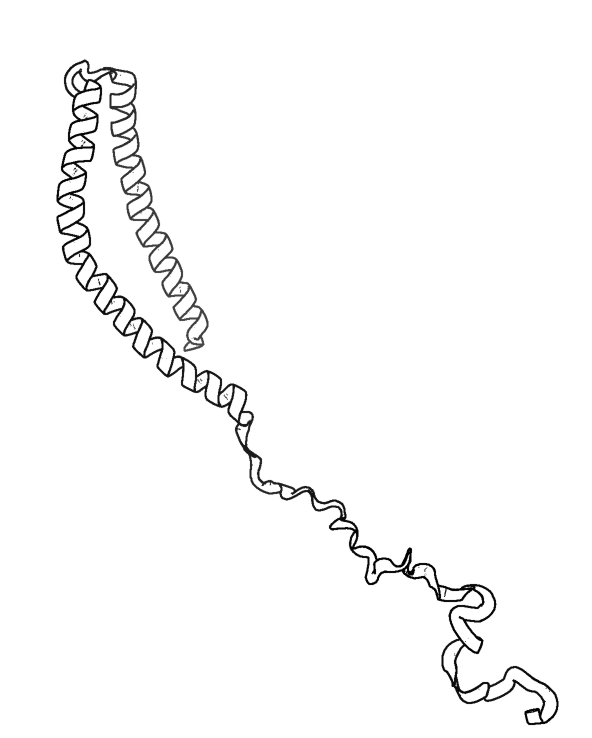
\includegraphics[width = \textwidth]{pics/alpha_struct.png}
		\caption{-конформация}\label{fig:alpha}
	\end{subfigure}
	\begin{subfigure}[t]{0.6\textwidth}
		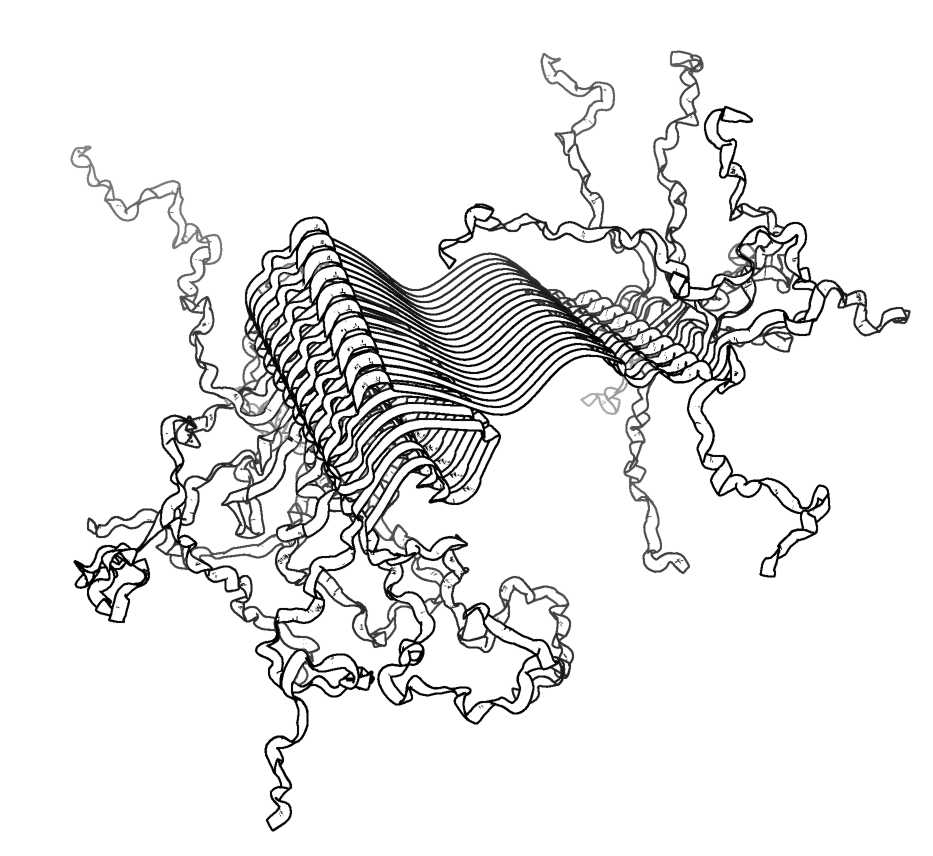
\includegraphics[width = \textwidth]{pics/beta_struct.png}
		\caption{конформация}\label{fig:beta}

	\end{subfigure}
	\caption{Конформации α-синуклеина.   
		(a) мембран-связанная, α-спиральная конформация, PDB ID: 1XQ8, \cite{ulmer_structure_2005};
		(b) фибриллы, аггрегированные \textbeta-листы, PDB ID: 2N0A, \cite{tuttle_solid-state_2016}.
		}
	\label{fig:structs}
	
\end{figure*}

Внутренне неструктурированные белки (известно около 100) обычно имеют амикислотную последовательность, которая препятствует агрегации и вообще формированию устойчивой конформации. Этому служит большое содержание заряженных остатков, пролина, отсутствие гирдрофобных стречей \cite{radivojac_intrinsic_2007}. 

В синуклеине такую роль выполняют N и C концевые домены, которые поддерживают белок в довольно компактном, динамическом состоянии, прикрывая NAC домен, так как он наиболее склонен в агрегации. Различные дальние (long-ranged) взаимодействия N и C доменов предотвращают агрегацию \cite{bertoncini_release_2005}.

Однако, различные мутации, пост-трансляционные модификации, изменения условий среды часто приводят к нарушению равновесия несвернутой конформации, заставляя белок фибрилизоваться.

Скорость образования фибрилл и олигомеров \textit{in vitro} линейно зависит от концентрации свободного растворенного белка, сильно ускоряется при наличии сформированных ядер нуклеации \cite{wood_-synuclein_1999}.





\subsubsection{Физиологическая роль}

Физиологическая роль α-синуклеина не ясна. Белки семейства синуклеинов были найдены только у позвоночных. 

α-Синуклеин, в основном, экспрессирован в мозге \cite{jakes_identification_1994} -- неокортексе, гиппокампе, стриатуме, таламусе, мозжечке \cite{iwai_precursor_1995}. Однако, также был найден в других тканях в сравнительно незначительных количествах. 

В отличие от других белков, ассоциированных с нейродегенерацией, синуклеин специфично локализуется в пресинаптических областях, его мало в теле нейронов, дендритах и в постсинаптических сайтах \cite{george_characterization_1995, iwai_precursor_1995}. 

Одна из ведущих концепций состоит в том, что  α-синуклеин выполняет функции в пресинаптических окончаниях нейронов и регулирует синаптическую передачу. В пользу этого говорит пресинаптическая локализация белка и его колокализация с резервным пулом пресинаптических везикул \cite{lee_-synuclein_2008}.

Тем не менее, в процессе развития синапсов синуклеин одним из последних колокализуется с синапсами, после интегральных белков синаптических пузырьков и синапсинов \cite{withers_delayed_1997}.

Аналогично α-синуклеину, β-синуклеин также локализуется пресинаптически \cite{jakes_identification_1994}. α- и  β- синуклеины действительно колокализуются, но не во всех синапсах. Однако, γ-синуклеин экспрессируется глиальными клетками и только в определенных нейрональных популяциях -- допаминэргических нейронов \cite{galvin_differential_2001}. γ-Синуклеин также экспрессируется в раковых опухолях (груди, прямой кишки, поджелудочной), где, возможно, играет роль в разрастании опухоли. 

 

Можно выделить следующие функции синуклеина:
\paragraph{Участие в липидном обмене и моделирование мембран} α-Синуклеин может служить переносчиком жирных кислот \cite{sharon_-synuclein_2001}.
Он также вызывает значительное искривление мембраны, превращая большие везикулы в трубочки и пузырьки  \cite{westphal_monomeric_2013} .
 
Биохимически α- и β-синуклеины были очищены как ингибиторы фосфолипазы D2 (PLD2) \cite{jenco_regulation_1998}. PLD2 гидролизует фосфатидилхолин до холина и фосфатидной кислоты и регулирует транспорт мембран, экзо- и эндоцитоз, организацию цитоскелета \cite{colley_phospholipase_1997}. В отличие от изоформы PLD1, которая активируется некоторыми клеточными каскадами, PLD2 обладает конститутивной активностью. Ингибиторная роль синуклеина была подтверждена в дрожжах \cite{outeiro_yeast_2003}, клетках млекопитающих \cite{ahn_-synuclein_2002}, \textit{in vitro}, причем была рассмотрена роль различных доменов белка в ингибировании, \cite{payton_structural_2004}. Однако, последние работы предполагают, что синуклеин не ингибирует PLD2 напрямую \cite{rappley_evidence_2009} и что данный эффект имеет причину гораздо более сложную, чем взаимодействие белков и может быть опосредован со эндоретикулярным стрессом.




\paragraph{Роль в везикулярном транспорте} Агрегаты синуклеина нарушают везикулярный транспорт в клетках млекопитающих \cite{gosavi_golgi_2002}. Мутации, связанные с БП, демонстрируют такой же эффект \cite{thayanidhi_alpha-synuclein_2010}. 

\paragraph{Регуляция обмена дофамина} Синуклеин подавляет экспрессию и активность тирозин редуктазы (ТР) -- фермент в пути биосинтеза дофамина \cite{yu_inhibition_2004} . Возрастное повышение экспрессии синуклеина коррелирует с понижением экспресии ТР \cite{chu_age-associated_2007} . Синуклеин нарушает обмен дофамина, ингибируя белок-переносчик дофамина в везикулах VMAT2 \cite{guo_inhibition_2008} .

\paragraph{Потенциальный шаперон} Синуклеин может иметь функции шаперона. Он структурно и функционально гомологичен 14-3-3 семейству шаперонов \cite{ostrerova_alpha-synuclein_1999}. С-концевой домен синуклеина подавляет аггрегацию термически денатурированных белков \cite{kim_structural_2002}. Синуклеин восстанавливает летальную делецию кошаперона CSPα в мышах, координируя сборку SNARE комплекса\cite{chandra_alpha-synuclein_2005} . Мыши -- тройные нокауты по синуклеинам демонстрируют ухудшение сборки SNARE-комплексов \cite{greten-harrison_-synuclein_2010}.

\paragraph{Выброс нейромедиатора и синаптичеcкая пластичность}
Синуклеин взаимодействует с синаптическими везикулами \cite{maroteaux_synuclein:_1988} и синаптобревином-2 \cite{burre_-synuclein_2010}, а также участвует в пересборке SNARE-комплексов как шаперон.
Уровень мРНК α-синуклеина (в этой работе названного синелфином "synelfin") значительно меняется в период обучения пению у певчих воробьиных \cite{george_characterization_1995}. Относительно всего мозга, где уровень синуклеина остается высоким на протяжение развития и взросления, в определенных областях, вовлеченных в пение, экспрессия синуклеина значительно и продолжительно падает, что предполагает участие белка с регулировке синаптической пластичности. 

Тем не менее α-cинуклеин нокаутные мыши живут нормально. У них наблюдается незначительное повышение выброса дофамина из нейронов вместе с понижением его содержания внутри клеток, нейроны быстрее восстанавливаются после нескольких стимуляций  \cite{abeliovich_mice_2000}. Двойные нокаутные мыши по α- и  β-синуклеинам также жизнеспособны, имеют нормальную морфологию мозга и синапсов, но уровень дофамина у них понижен \cite{chandra_double-knockout_2004}. Тройные нокауты, однако, демонстрируют меньший срок жизни, возрастные дисфункции нервной системы, изменение морфологии синапсов -- уменьшение размеров пресинаптических терминалей \cite{greten-harrison_-synuclein_2010}.

Учитывая специфичность синуклеина для позвоночных, а также позднюю локализацию около синапсов, можно предполагать, что он не является ключевым фактором их развития, хотя и влияет на функционирование в долгосрочной манере. 



\subsection{Патобиология α-синуклеина}

В 1977 было обнаружено, что α-синуклеин -- основной компонент телец и невритов Леви \cite{spillantini_-synuclein_1997} -- белковых клеточных включений, которые являются одним из основных признаков болезни Паркинсона (БП) и деменции с тельцами Леви (ДТЛ) -- что получило названии патологии Леви. 

Деменция с тельцами Леви очень похожа на идиопатические случаи БП по нейропатологии, при этом клинические проявления болезни другие. %ДТЛ характеризуется когнитивным растройством, паркинсонизмом, резкими колебаниями внимания и интеллекта и визуальными галлюцинациями.

α-Синуклеин также вовлечен в множественную системную атрофию (МСА).
В МСА α-синуклеин накапливается в глиальных клетках -- олигодендроцитах. Экспрессия синуклеина в таких культурах воспроизводит фенотип МСА, что позволяет считать синуклеин причиной патологии. В норме олигодендроциты не экспрессируют синуклеин, что поднимает вопрос -- как белок оказывается в клетках, захватывает ли глия белок из нейронов или экспрессия активируется неким патологическим процессом? При этом наследственные формы МСА очень редки \cite{bendor_function_2013}.

Синуклеин также вовлечен в другие нейродегенеративные заболевания -- первичную вегетативную недостаточность, диффузную болезнь Леви, нейродегенерацию с аккумуляцией железа типа I \cite{burre_cell_2018}. Около 60\% случаев болезни Альцгеймера сопровождаются патологией Леви, которая, однако, обычно обнаруживается только в миндалевидном теле \cite{hamilton_lewy_2006}.

\subsubsection{Болезнь Паркинсона}
Болезнь Паркинсона -- нейродегенеративное заболевание, которое оюнаруживается у 2-3\% населения старше 65 лет \cite{poewe_parkinson_2017}, в мире с этим заболеванием живут около 10 миллионов человек (данные Parkinson’s Foundation). 

Основные признаки БП -- потеря нейрональных функций в некоторых областях мозга и широкое внутриклеточное накопление α-синуклеина. Потеря допаминэргических нейронов на ранних стадиях ограничена черной субстанцией, но далее наблюдается в других частях мозга. 
Патология Леви обнаруживается в холинэргических и моноаминэргических нейронах ствола мозга и в нейронах обонятельной системы, с прогрессией заболевания -- в либмической системе и неокортексе.

Большинство случаев БП -- идиопатические с поздним началом, генетически обусловлены около 5-10\% патологий \cite{klein_genetics_2012}. 

Ду- или трипликации гена синуклеина обуславливают БП с ранним началом  и значительной деменцией \cite{chartier-harlin_alpha-synuclein_2004, ahn_-synuclein_2008, singleton_-synuclein_2003}. Некоторые полиморфизмы в регуляторных элементах гена синуклеина также ассоциированы с БП с ранним началом \cite{maraganore_collaborative_2006}.

Некоторые мутации миссенс α-синуклеина ассоциированы с классическим проявлением БП, наследуются по аутосомно-доминантному типу: A30P \cite{kruger_ala30pro_1998}, E46K \cite{zarranz_new_2004}, H50Q \cite{appel-cresswell_alpha-synuclein_2013}, G51D\cite{lesage_g51d_2013}, A53T\cite{puschmann_swedish_2009}, A53E \cite{pasanen_novel_2014} (OMIM entry 163890).

 Все они расположены в N-концевом домене белка. Мутация A30P ухудшает связывание синуклена с мембранами \cite{jo_defective_2002}, E46K -- повышает сродство к мембранам и ускоряет агрегацию \cite{choi_mutation_2004}, H50Q -- понижает растворимость \cite{porcari_h50q_2015}. Интересно заметить, что у грызунов в позиции 53 в норме находится треонин (для людей мутация A53T токсична) и БП не наблюдается.
 
 
Другие гены, ассоциированные с наследуемыми, моногенными формами БП -- богатая лейцином повторная киназа 2 (leucine-rich repeat kinase 2, LRRK2) , Е3 убиквитин лигаза Паркин (Parkin), митохондриальная PTEN-индуцируемая киназа 1 (Pink1), шаперон DJ-1, лизосомная АТФаза ATP13A2 \cite{klein_genetics_2012}.


Не ясно, как именно дегенерация нервных клеток в БП соотносится с аккумуляцией синуклеина.  
В черной субстанции потеря нейронов может наступать раньше появления моторных синдромов. Сама по себе патология Леви не всегда сопровождается потерей клеток -- ведь синуклеин накапливается по всему мозгу. Более того, накопление синуклеина может и не приводить ни к какой патологии \cite{markesbery_lewy_2009}. Возможно, синуклеин играет защитную роль, тогда как его мутантные форму приводят к дисфункции \cite{bendor_function_2013}.



\subsection{Моделирование токсичности синуклеина на дрожжах \emph{S.cerevisiae}}

Пекарские дрожжи \emph{Saccharomyces cerevisiae} не имеют ортологов синуклеина. Тем не менее, они используются как удобная модель для изучения синуклеина.

Такая простая модель имеет свои недостатки -- например, на дрожжах невозможно смоделировать клеточные взаимодействия, которые присутствуют в тканях многоклеточных, не говоря уже о нервных синапсах, в образовании и функционировании которых синуклеин может принимать участие. Тем не менее, участие синуклеина во внутриклеточных каскадах и взаимодействие с другими белками может быть широко изучено на дрожжах, которые легко поддаются генетическим манипуляциям.

Первая модель БП была основана на гетерологической экспрессии синуклеина в дрожжах \cite{outeiro_yeast_2003}.

Токсичность синуклеина в дрожжах зависит от уровня его экспрессии \cite{outeiro_yeast_2003}, что согласуется с существованием форм БП, вызванных ду- и трипликациями гена синуклеина.

Также α-синуклеин ассоциируется с плазматической мембраной, куда доставляется системой секреции \cite{dixon_-synuclein_2005}. Накопление белков, ассоциированных с мембраной, ведет к образованию цитоплазменных включений в концентрационно-зависимой манере \cite{dixon_-synuclein_2005}. 

Аналогично тельцам Леви в мозге с БП, многие включения α-синуклеина в клетках дрожжей окрашиваются тиофлавином-S, следовательно содержат амилоидные фибриллы \cite{zabrocki_phosphorylation_2008}, и тиофлавином Т \cite{oien_clearance_2009}. Было также продемонстрировано, что в клетках дрожжей образуются и олигомеры синуклеина \cite{tenreiro_phosphorylation_2014}.
При этом некоторые включения представляют собой агрегированные мембранные пузырьки \cite{soper_-synucleininduced_2008}.

Дрожжи понижают среднее число  мультикопийных плазмид с синуклеином на клетку, вероятно, для подавления его токсичности \cite{outeiro_yeast_2003}. Во избежание этого, для поддержания высокого уровня экспрессии, последовательность синуклеина интегрируется в геном в разном числе \cite{cooper_-synuclein_2006, su_compounds_2010}, либо используются сильные промоторы, например, галактозный GAL1 \cite{outeiro_yeast_2003}.

 Экспрессию синуклеина сопровождает митохондриальный стресс \cite{su_compounds_2010}. 
При этом система экспрессии под контролем промотора MET25 показала, что для проявления токсичности синуклеина необходимы функционирующие митохондрии \cite{buttner_functional_2008}.  

Оверэкспрессия синуклеина в дрожжах вызывает нарушение работы протеасомной системы \cite{outeiro_yeast_2003}, 
	накопление липидных капель \cite{outeiro_yeast_2003},
	стресс эндоплазматического ретикулума \cite{cooper_-synuclein_2006},
	активацию ответа на тепловой шок \cite{yeger-lotem_bridging_2009},
	дисфункцию митохондрий \cite{su_compounds_2010},
	укорочение срока жизни и индукцию митофагии \cite{sampaio-marques_snca_2012},
	нарушение эндоцитоза \cite{outeiro_yeast_2003},
	выделение активных форм кислорода и индукцию апоптоза \cite{su_compounds_2010, flower_ygr198w_2007}. 
	Было показано, что апоптоз вызывается транслокацией эндонуклеазы~G из митохондрий в ядро, где она осуществляет деградацию ДНК \cite{buttner_endonuclease_2013}.
	

В дрожжах найдено 4 гомологичных и высококонсервативных гена, принадлежащих суперсемейству DJ-1:  Hsp31, Hsp32, Hsp33 и Hsp34. Человеческий белок DJ-1, оверэкспрессированный в дрожжах, взаимодействует с синуклеином, а мутации в DJ-1, связанные с болезнью Паркинсона, нарушают это взаимодействие. DJ-1 и его гомологи в дрожжах снижали токсичность синуклеина, препятствуя его олигомеризации \cite{zondler_dj-1_2014}. 



\subsubsection{Скрининги}

Дрожжи являются удобным объектом для проведения генетических скринингов.

В первом проведенном скрининге использовалась коллекция из 4850 делеционных штаммов \cite{willingham_yeast_2003}. Было определено 86 генов, которые увеличивают токсичность синуклеина, из которых 29\% вовлечены в везикулярный транспорт и метаболизм липидов.
Особо отметим четыре гена -- VPS24, VPS28, VPS60 or SAC2 -- делеция которых увеличивала токсичность синуклеина. Они вовлечены в сортировку белков в поздних цистернах Гольджи и доставку в вакуоли. 

 Позже, с использованием той же коллекции и применением флуоресцентной микроскопии, было выявлено 185 модификаторов агрегации синуклеина \cite{zabrocki_phosphorylation_2008}. Выяснилось, что белки, регулирующие везикулярный транспорт, меняют локализацию синуклеина в клетке.

В оверэкспрессионной скрининге было обнаружено, что синуклеин блокирует транспорт от эндоплазматического ретикулума к аппарату Гольджи (ER-to-Golgi) \cite{cooper_-synuclein_2006}. Это привело к обнаружению белка Rab1, гомолога белка млекоптающих Ypt1, который оказался нейропротектором, который восстанавливает ER-to-Golgi транспорт в дрожжах, а его близкие гомологи восстанавливают здоровый фенотип нейронов с БП в различных животных моделях -- в нервной системе нематоды и в первичной культуре нейронов крысы с БП \cite{gitler_parkinsons_2008}.

Ypp1 -- жизненно необходимый белок дрожжей с неизвестной функцией,  как оказалось, при оверэкспресии опосредует транспорт синуклеина (мутантного, A30P) в вакуоли по эндоцитозному пути и, таким образом, восстанавливает нормальный фенотип клеток \cite{flower_ygr198w_2007}.


Оверэкспрессия 40 генов подавляет повышенную чувствительность дрожжей, экспрессирующих синуклеин, к действию пероксида водорода, что говорит о защитной функции этих генов против токсичности синуклеина \cite{liang_novel_2008}. Найденные гены вовлечены в убиквитин-зависимый катаболизм белков, везикулярный транспорт, ответ на стресс. 

Среди генов, отмеченных исследователями -- ARG2, ENT3, IDP3, JEM1 -- не жизеннно важные и имеют человеческих ортологов, показали наибольшую защитную функцию от активных форм кислорода, а HSP82 кодирует широко распространенный шаперон (Hsp90p). 
	Arg2p -- митохондриальный фермент, который катализирует первую реакцию в биосинтезе орнитина. Ent3p вовлечен в связывание клатрина и транспорт белков между транс-Гольджи и вакуолью. Idp3p -- пероксисомный вариант изоцитратдегидрогеназы. Jem1p -- шаперон, локализованный на эндоплазматическом ретикулуме, участвует в слиянии ядерных мембран при спаривании. Оказалось, что делеция данных генов действительно ухухдшает выживаемость дрожжей при экспрессии синуклеина.


Комплексное исследование взаимодействия синуклеина с различными клеточными путями, с использованием коллекции из 3500 штаммов, оверэкспрессирующих различные белки, позволило составить карту белков и генов, связанных с экпрессией синуклеина в клетке. Путь биосинтезе эргостерола и TOR каскад, как было найдено, влияют на эффекты, оказываемые синуклеином в дрожжах \cite{yeger-lotem_bridging_2009}.














































        \begin{table}[h]
	\small
	\caption{}
	\label{table:}
	\begin{tabular}{p{0.3\width}}
	\graytable
	\toprule
	\midrule
	\bottomrule
	\end{tabular}
\end{table}




\section{Материалы и методы}
\subsection{Материалы}



\subsubsection{Использованные штаммы микроорганизмов}
\label{subsec:strains}

Штаммы дрожжей и бактерий описаны в таблице~\ref{table:strains}.

Использованные родительские штаммы были взяты из коллекции лаборатории. Созданные штаммы также архивировали, суспендируя свежие клетки в 1\,мл стерильного 20\%\,глицерина, затем хранили при -70 ºС.

Штамм cdc53-1 -- термочувствительный мутант, который растет и делится при пермесивной температуре 25°C, но аррестуется в фазе G\textsubscript{0} при 37°C \cite{mathias_cdc53p_1996}. Белок Cdc53 -- компонент убиквитин-лигазной системы, которая направляет фосфорилированные циклины  G\textsubscript{0} (Cln1, Cln2, Cln3) на протеасомную деградацию \cite{willems_cdc53_1996}. Точнее, это каркасный белок различных комплексов Cdc34/Skp1/F-box, которые участвуют в регуляции клеточного цикла и синтеза метионина \cite{patton_cdc53_1998}, а мутация cdc53-1, возможно, даже нарушает целосность клеточной стенки дрожжей \cite{varelas_cdc34/scf_2006}.

\begin{table}[p]
	\small
	\caption{Описание штаммов дрожжей и бактерий, использованных в работе.}
	\label{table:strains}
	\begin{tabular}{ p{0.25\width - \tabcolsep} p{0.65\width - 2\tabcolsep}  p{0.1\width - \tabcolsep}}
		\graytable
		\toprule
		Название штамма & Описание & Источ-ник \\ 
		\midrule
		
		\multicolumn{3}{l}{ \textit{Saccharomyces cerevisiae} }\\
		\invisiblerule
		W303 &
			MAT\textbf{a} ade2-101 his3-11 trp1-1 ura3-52 can1-100 leu2-3,112, GAL, psi+ &
			$^1$ \\  \invisiblerule
		cdc53-1 &
			MAT\textbf{a} ade2-1 his3-11 trp1-1 ura3-52 can1-100 leu2-3,112,15 cdc53-1 &
			$^1$ \\  \invisiblerule
		W303-1a::URA3 &
			 MAT\textbf{a} ade2-101 his3-11 trp1-1 URA3 can1-100 leu2-3,112, GAL, psi+&
			$^1$ \\  \invisiblerule
		диплоид &  
			diploid ade2-101 his3-11 trp1-1 ura3-52 can1-100 leu2-3,112, GAL, psi+ 
			& $^1$\\   \invisiblerule
		W303/αSyn &  W303-1a, плазмида p426GALaSynGFP & $^2$\\  \invisiblerule
		cdc53-1/αSyn &  cdc53-1, плазмида p426GALaSynGFP & $^2$ \\  \invisiblerule
		W303/αSyn/LEU2 &  W303-1a, плазмиды p426GALaSynGFP и YEp13 & $^2$ \\  \invisiblerule
		cdc53-1/αSyn/LEU2 &  cdc53-1, плазмиды p426GALaSynGFP и YEp13 & $^2$\\  \invisiblerule
		W303::URA3/LEU2& W303-1a::URA3, плазмида YEp13 & $^2$ \\
		
		\midrule
		\multicolumn{3}{l}{\textit{Escherichia coli} }\\ \invisiblerule
		E.coli XL1 Blue &
		recA1 endA1 gyrA96 thi-1 hsdR17 supE44 relA1 lac [F' proAB lacI\textsuperscript{q}Z$\Delta$M15 Tn10 (Tet\textsuperscript{r})]&
		\scriptsize{EvroGen\texttrademark} \\
		
		
		\bottomrule
	\end{tabular}
	\begin{tabular}{p{1\width}}
			$^1$ коллекция лаборатории \\
			$^2$ штаммы были получены из приведенных введением плазмид
			\\
	\end{tabular}
	
\end{table}





\subsubsection{Плазмиды и библиотеки} 
\label{subsec:libs}

Плазмиды, использованные в данной работе, охарактеризованы в таблице~\ref{table:plasmids}. 

Плазмида p426GALaSynGFP \cite{outeiro_yeast_2003} использовалась для экспрессии и изучения гибридного белка -- α-синуклеина, слитого с GFP. Карта плазмиды приведена на рисунке~\ref{fig:plasmid}.


\begin{table}[p]
	\small
	\caption{Плазмиды, использованные в работе.}
	\label{table:plasmids}
	\begin{tabular}{ 
		p{0.3\width - \tabcolsep}
		p{0.55\width - 2\tabcolsep} 
		p{0.15\width - \tabcolsep} }
	\graytable
	\toprule
	Плазмида & Описание & Источник \\ \midrule

	p426GALaSynGFP  &
		2$\mu$, URA3, ampR, экспрессия α-синуклеина-GFP&
		\cite{outeiro_yeast_2003} \\
	pYES-DA-6 &
		2$\mu$, URA3, ampR & $^1$ \\
	pYES2 &
		2$\mu$, URA3, ampR & $^1$\\	
	YEp13 &
		2$\mu$, LEU2, ampR & $^1$ \\
	pRS314 &
		CEN/ARS, TRP1, ampR & $^1$\\

	\bottomrule
	\end{tabular}
	\begin{tabular}{p{1\width}}
			$^1$ коллекция лаборатории \\
	\end{tabular}
	
\end{table}

\begin{figure}[p]
	\centering
	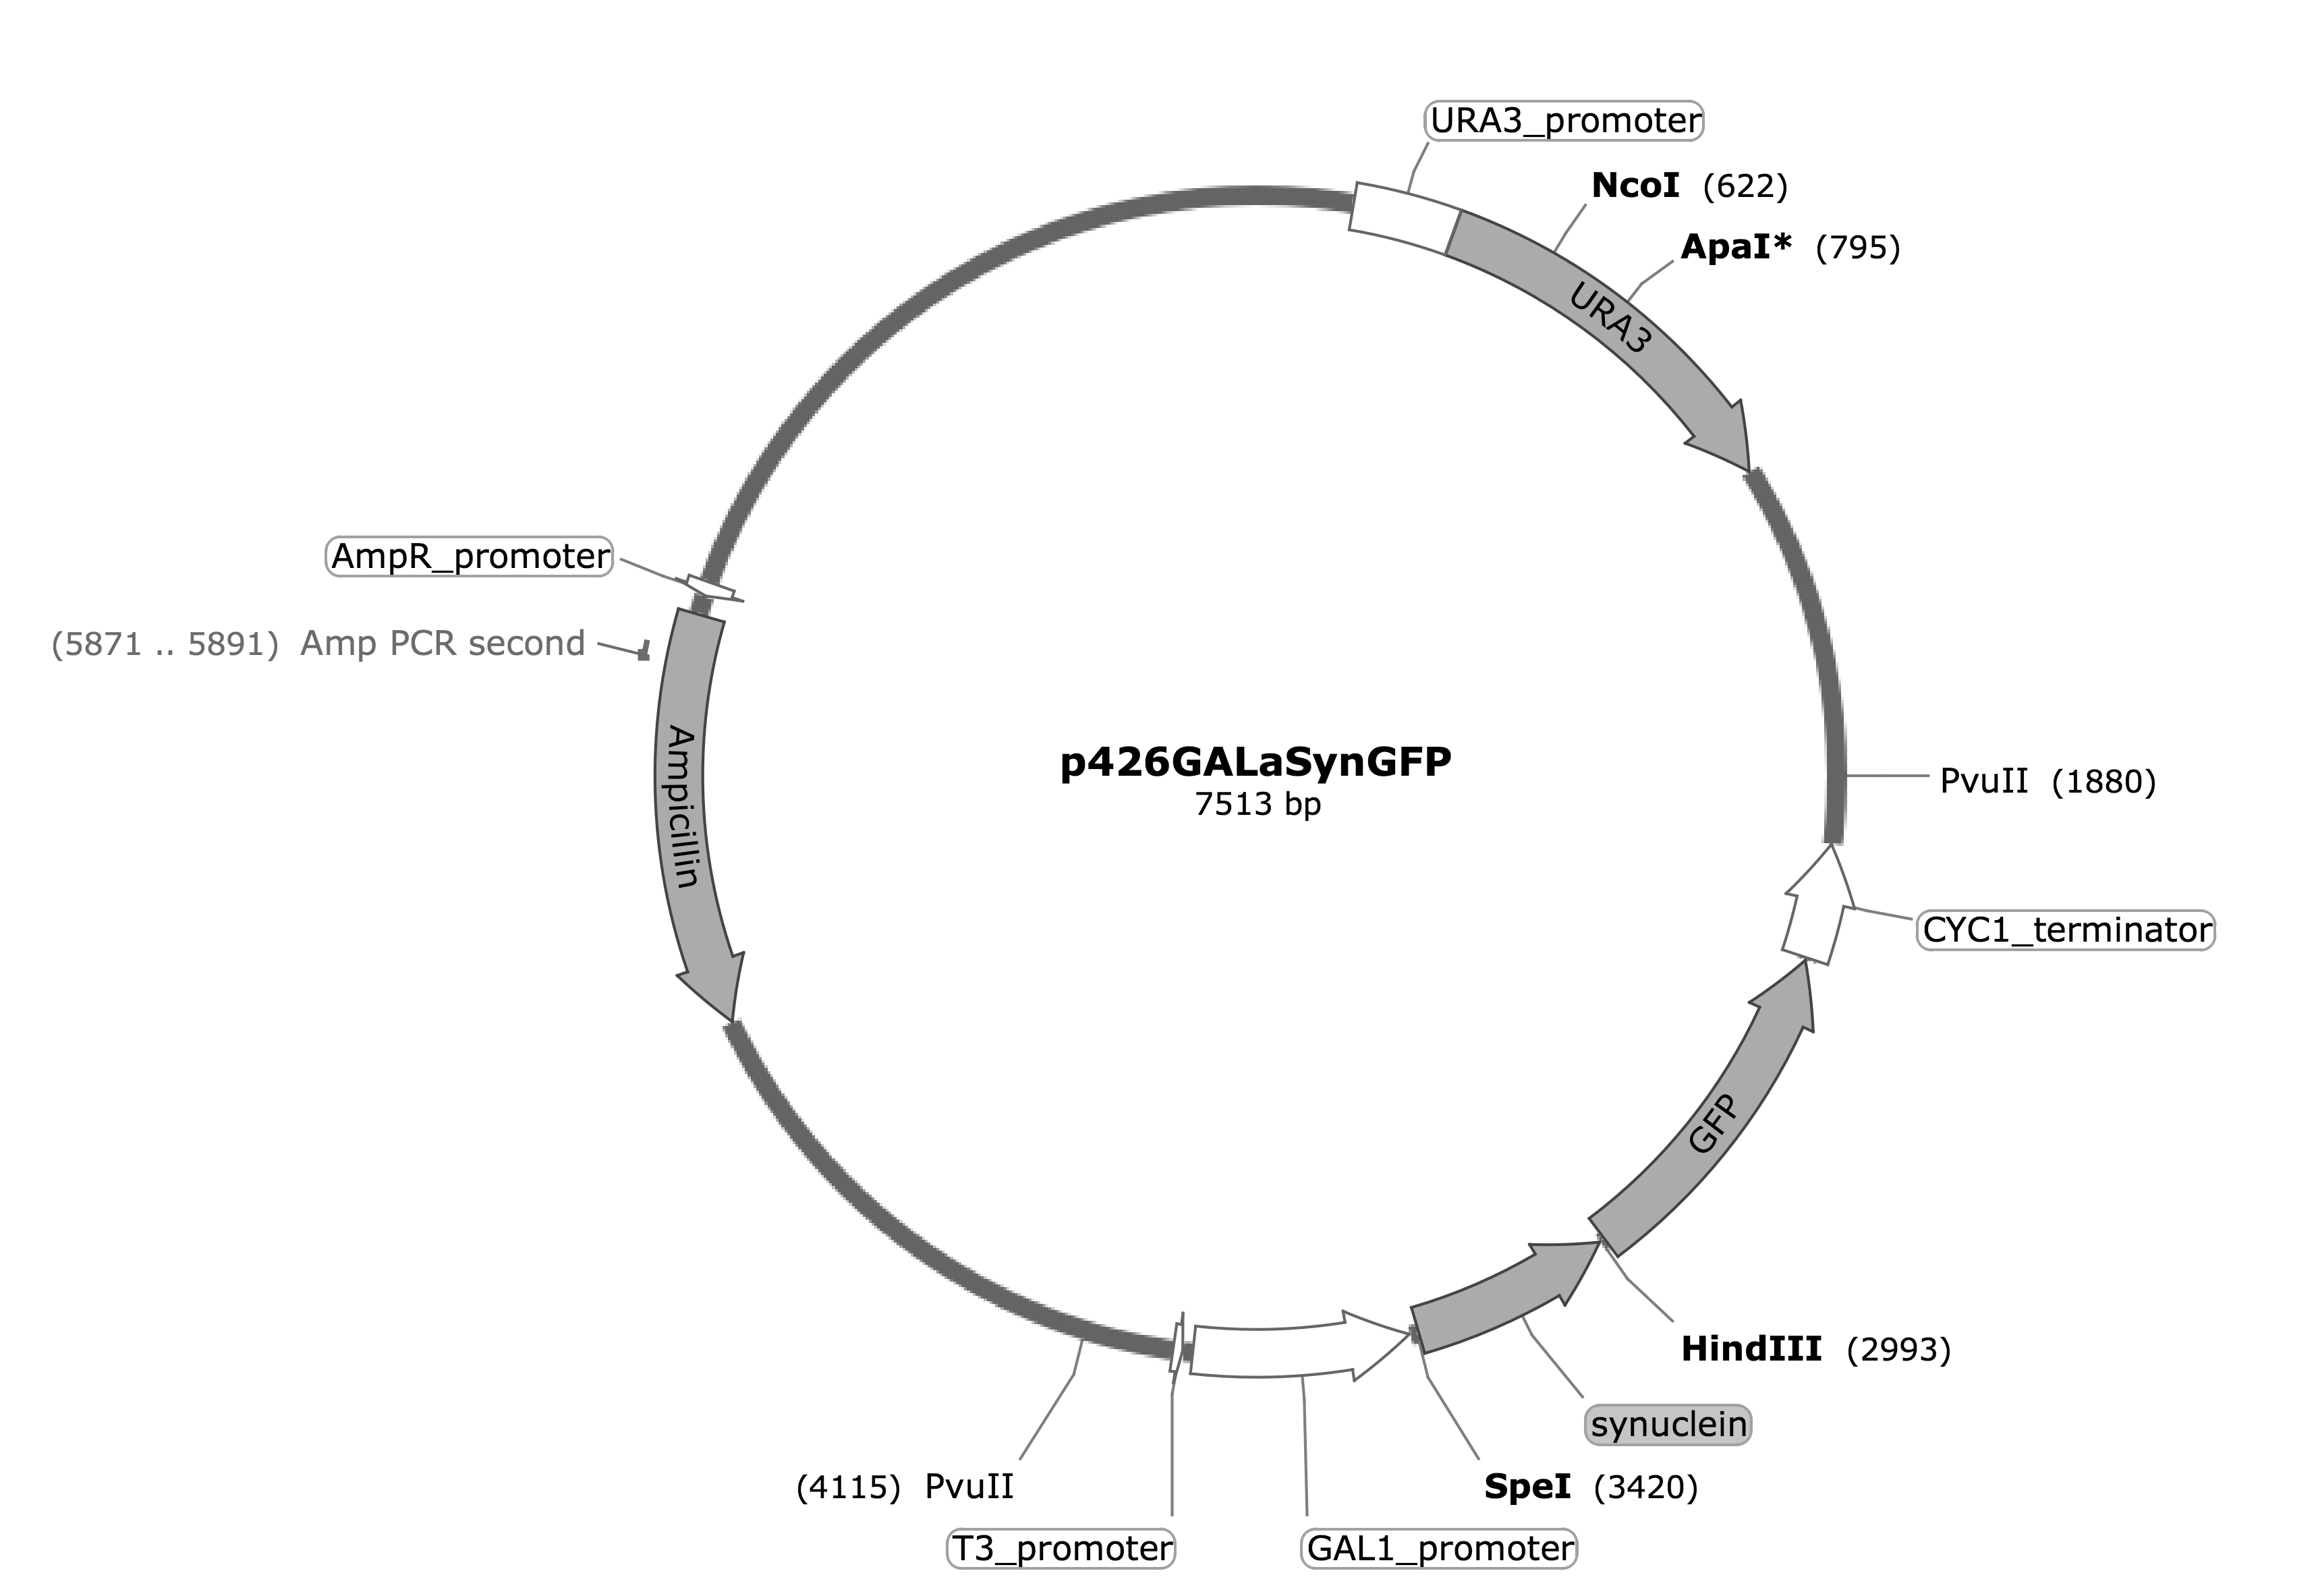
\includegraphics[width = 0.85\textwidth]{pics/p426GALaSyn_Map}
	\caption{Карта плазмиды p426GALaSynGFP, которая использовалась для экспрессии гибридного белка α-синуклеина-GFP в дрожжах. \gray{Точная нуклеотидная последовательность плазмиды нам была не известена, данная карта составлена на основе описания \cite{outeiro_yeast_2003} } }
	\label{fig:plasmid}	
\end{figure}


Геномные библиотеки, которые использовались для скринина, представлены в таблице~\ref{table:libs}.

Сверхэкспрессионная --  эписомальная, мультикопийная библиотека YEp13\,lib, используется в виде плазмид.
Делеционная -- библиотека lib25 \cite{burns_large-scale_1994}. Lib25 представляет из себя геномную библиотеку дрожжей, лигированную в вектор pHSS6, в которую далее был встроен транспозон mini-Tn3::LEU2, использовалась в виде продукта рестрикции по уникальному сайту NotI(см. \ref{sec:restriction}).

\begin{table}[p]
	\small
	\caption{Геномные библиотеки, использованные в работе.}
	\label{table:libs}
	\begin{tabular}{p{0.4\width - \tabcolsep}p{0.3\width - 2\tabcolsep}p{0.3\width - \tabcolsep}}
	\graytable
	\toprule
	&YEp13 lib& Lib25 \\
	\midrule
	Тип & 
		эпимсомальная, мультикопийная, оверэкспрессионная & 
		делеционная \\ \thinrule
	Исходный вектор & YEp13 & pHSS6\\ \thinrule
	Исходный размер вектора & 10.7\,kb & 2,5\,kb\\ \thinrule
	Размер фрагментов геномной ДНК дрожжей & 5-20\,kb & 1,9-3,5\,kb (в среднем 3kb)\\ \thinrule
	Маркёры & LEU2, ampR & LEU2, ampR \\ \thinrule
	
	Количество клонов для покрытия генома дрожжей & $1.0\times10^4$ & $3.0\times10^4$ \\ \thinrule
	Число независимых рекомбинантов (вариантов вектора) & $8.2\times10^4$ & $>10^5$ \\ \thinrule
	Источник & 
		\footnotesize{ \textit{Saccharomyces cerevisiae} (ATCC\textregistered 37323\texttrademark)} &
		\cite{burns_large-scale_1994} \\
	\bottomrule
	\end{tabular}
\end{table}





\subsection{Культивирование}
\subsubsection{Условия культивирования}
Микроорганизмы растили на питательных средах различного состава (таблица~\ref{table:mediums}) в термостате (на твердой агаризованной среде на чашках Петри) или термостатируемой качалке (на жидкой среде в колбах и 50 мл пробирках типа «Falkon», обязательное перемешивание 250 rpm). Оптимальная температура роста для дрожжей --  30 ºС (для не термочувствительных штаммов) или  25 ºС (для термочувствительных мутантов cdc53). Бактерии растили при 37 ºС.


\subsubsection{Среды для культивирования}
Питательные среды, использовавшиеся для культивации дрожжей и бактерий, перечислены в таблице~\ref{table:mediums}. Бактерии растили в LB. Дрожжи дикого типа растили на натуральной среде (YPD), мутантов, содержащих плазмиды с селективными маркёрами -- на соответствующих синтетических селективных средах (YNB).

В твердые среды добавлялся агар. Среды стерилизовали автоклавированием при 2 атм. 121 ºC в течение 50 минут. Растворы сахаров автоклавировали отдельно, затем смешивали со средой. Антибиотики добавляли в среды после автоклавирования. 

\begin{table}[p]
	\footnotesize
	\caption{Состав сред для культивирования}
	\label{table:mediums}
	\begin{tabular}{ p{0.3\width - \tabcolsep} p{0.55\width - 2\tabcolsep} p{0.15\width - \tabcolsep} }
	\graytable
	\toprule
	Название & Состав & \\
	\midrule
	LB & 
		LB \scriptsize (триптон 10г, дрожжевой экстракт 5г, NaCl 10г)& 25 г/л\\
		& (агар) & 20 г/л\\

	\thinrule
	LB Amp & 
		LB & 25 г/л\\
		& (агар) & 20 г/л\\
		& ампицилин & 0.1 г/л\\
	\thinrule
	SOC & 
		LB & 25 г/л \\
		&МgCl\textsubscript{2} & 5 мМ\\
		&MgSO\textsubscript{4} & 5 мМ\\
		&глюкоза& 10 г/л\\
	YPD & 
			дрожжевой экстракт & 10 г/л \\ 
			& пептон  & 20 г/л\\
			& D-глюкоза & 20 г/л \\
			& (агар) & 20 г/л \\
			
	\thinrule
	YNB selective D/GAL & 

			YNB (yeast nitrogen base) &  6.6 г/л\\
			&селективная аминокислотная добавка (табл.~\ref{table:dropout}) & ...\\
			&D-глюкоза / D-галактоза & 20 г/л \\
			&(агар) & 20 г/л \\


	\bottomrule
	\end{tabular}
\end{table}

\begin{table}[p]
	\footnotesize
	\caption{Аминокислотные добавки для селективных сред}
	\label{table:dropout}
	\begin{tabular}{p{0.3\width - \tabcolsep} p{0.6\width - 2\tabcolsep} p{0.1\width - \tabcolsep}}
	\graytable
	\toprule
	Селективная среда & Аминокислотная добавка & \\
	\midrule
	-ura & Yeast Synthetic Drop-out Medium Supplements without (YSDMS w/o) uracil & 1.92 г/л\\
	\thinrule
	-leu & YSDMS w/o leucine  & 1.6 г/л\\
	\thinrule
	-ura-leu & YSDMS w/o histidine, leucine, tryptophan and uracil  & 1.4г/л \\
		& L-histidine & 20 мг/л \\
		& L-tryptophan & 20 мг/л \\
		\\
	
	\bottomrule
	\end{tabular}
\end{table}



\subsection{Молекулярно-биологические методы}


\subsubsection{Подготовка компетентных бактериальных клеток}
\label{subsec:bac_comp}

Компетентные клетки для электропорации готовили из электрокомпетентных клеток EvroGen\texttrademark E.coli XL1 Blue.
 
\begin{enumerate}[nolistsep]
	\item Клетки растили ночь в больших колбах (3-4 штуки) в LB при 30ºC и перемешивании 200\,rpm. Заранее охлаждали mQ и 10\% глицерин. 
	\item Через 12 часов измеряли оптическую плотность клеток при 595\,нм и доводили ее до 0.1-0.2 о.е. Растили при температуре 18ºC и перемешивании 6 часов в тех же колбах в LB (по 200\,мл).
	\item  Центрифугированили при температуре 4ºC  2200\,g 7\,мин. Промывали клетки холодной (4ºC) mQ (по 20 мл) 3 раза. Промывали клетки 10\% глицерином (20\,мл). 
	\item Ресуспендировали клетки в остатках глицерина (около 2\,мл). Аликвотировали в холодные пробирки по 50\,млкл. Замораживали в жидком азоте. Хранили при -70ºC.

\end{enumerate}

\subsubsection{Трансформация бактериальных клеток}
\label{subsec:bac_tranform}

Трансформацию бактериальных клеток \emph{Escherichia coli} проводили методом электропорации.

Для трансформации аликвоту компетентных клеток оттаивали во льду 20\,минут, добавляли ДНК, смесь перемешивали, инкубировали во льду (4ºC 10\,мин) и переносили в холодную кювету для электропорации, подвергали действию электрического разряда (1800\,В), после чего добавляли 500\,мкл SOC, инкубировали (37 ºС 60 мин при перемешивании 700\,rpm), сеяли на чашку(чашки) с селективной средой и растили ночь в термостате при 37 ºС.

\subsubsection{Выделение плазмидной ДНК из бактерий}
\paragraph{Выделение плазмид}
\label{subsec:bac_plasm_pur}
\begin{enumerate}[nolistsep]
	\item Для выделения плазмид одну колонию с чашки транформированных бактерий или небольшое число клеток из архива суспендировали в 2-3\,мл жидкой селективной среды и растили ночь при 37ºС.
	\item Ночную культуру охлаждали  в  течение  15\,мин  на  льду, центрифугировали (1400\,g 2\,мин), ресуспендировали в 250\,мкл охлажденной деионизованной воды и переносили на лед. 
	\item Добавляли 500\,мкл лизирующего буфера В (0,2\,M NaOH, 1\%\,SDS), аккуратно перемешивали, инкубировали (25ºС 3\,мин).
	\item Затем добавляли 350\,мкл нейтрализующего буфера С (5М ацетат калия, pH 7), встряхивали,  инкубировали (25ºС 15\,мин), затем центрифугировали (17000\,g 5\,мин). 
	\item Отбирали супернатант, содержащий плазмидную ДНК. 
	\item Добавляли 0,6 объема изопропанола, инкубировали во льду (4ºС 10\,мин), центрифунировали (17000\,g 5\,мин).
	\item Убирали супернатант, днк в осадке. Добавляли 500\,мкл mQ, 300\,мкл 9\,М ацетата аммония (NH\textsubscript{4}Ac), инкубировали в морозилке (-20ºС 5\,мин) и затем в холодильнике (4ºС 15\,мин), центрифунировали (17000\,g 5\,мин).
	\item Отбирали супернататант, добавляли 0,6 объема изопропанола, инкубировали во льду (4ºС 10\,мин), центрифунировали (17000\,g 5\,мин).
	\item Промывали ДНК этанолом: сливали изопропанол, добавляли 0,2,\,мл 70\%\,этанола, центрифунировали (2500\,g 2\,мин), убирали этанол.
	\item Подсушивали и растворяли в 100\,мкл деионизированной воды с небольшим добавлением РНКазы H(0,1\,мкл на 1\,мл воды).

	\end{enumerate}
	
\paragraph{Выделение плазмидных библиотек}
\label{subsec:bac_plasm_kit}
Для амплификации библиотек трансформированные бактерии высевали на большое число селективных чашек (10), растили ночь при температуре 37ºС. Контролировали число полученных клонов -- оно должно было превышать число клонов, необходимых для покрытия генома данной библиотеков (табл.~\ref{table:libs} и раздел \ref{subsec:libs}). Затем смывали колонии водой, выделяли и переосаждали плазмидную ДНК с помощью набора QIAGEN\textregistered Plasmid Purification Midi Kit.

\subsubsection{Переосаждение ДНК}
\label{subsec:dna_prec}

Переосаждение ДНК из раствора проводили на льду следующим образом: подсаливали раствор до 0.2\,М NaCl, добавляли 2.5\,объема спита EtOH 100\%,  инкубировали (30\,мин), центрифугировали (17000\,g 5\,мин), сливали супернатант, добавляли спирт EtOH 70\%, центрифугировали (17000\,g 5\,мин), сливали супернатант, высушивали, растворяли ДНК в воде.

\subsubsection{Обработка ДНК эндонуклеазами рестрикции} \label{sec:restriction}
	Для анализа различных образцов ДНК проводили рестрикцию различными эндонуклеазами рестрикции. Рестрикционную смесь готовили на основе деионизированной воды, десятикратного рестрикционного буфера, образца ДНК, рестриктазы.
	
	Рестрикцию плазмид или библиотек для последующего анализа на геле проводили в объеме 10\,мкл, используя 1-2\,мкл плазмиды и 0.2\,мкл фермента в течение 1-2\,часов при 37ºС.
	
	Рестрикцию делеционной библиотеки lib25 для дальнейшего использования проводили в объеме 120\,мкл, используя 30\,мкл библиотеки и 5\,мкл фермента NotI в течение 2-3\,часов при 37ºС с последующим переосаждением.

\begin{table}[!h]
	\small
	\caption{Эндонуклеазы рестрикции, использованные для анализа плазмид}
	\label{table:}
	\begin{tabular}{
		p{0.4\width - \tabcolsep}
		p{0.6\width - \tabcolsep}}
	\graytable
	\toprule
	Плазмида & Анализ рестриктазами\\
	\midrule
	p426GALaSynGFP & ApaI, HindIII, NcoI, PvuII, SpeI (рис.~\ref{fig:plasmid}) \\
	библиотека YEp13 & Eco32(EcoRV) (0.96, 3.3 kbp, inserts)\\ 
	делеционная библиотека lib25 & NotI(unique) \\
	pYes-DA-6 & Eco32(EcoRV) (unique)\\
	YEp13 &  Eco32(EcoRV) (0.96, 3.3, 6.4 kbp) \\
	pRS314 & Eco32(EcoRV) (1.2, 3.6 kbp) \\

	\bottomrule
	\end{tabular}
\end{table}	

\subsubsection{Горизонтальный гель-электрофорез ДНК}
\label{subsec:gel}
Для определения количества и размеров фрагментов ДНК использовали горизонтальный электрофорез в агарозном геле в присутствии бромистого этидия. Использовали гель на основе буфера ТАЕ (40мМ трис-ацетат (рН\,8.2), 20\,мМ ацетат натрия, 2\,мМ ЭДТА) с 1\% агарозы и бромистым этидием (0.5\,мг/мл) . Наносимые образцы предварительно смешивали с буфером для внесения (6x Loading Buffer - 0,25\%\,бромфеноловый синий, 0,25\%\,ксиленцианол, 30\%\,глицерин на воде).

Для рестрикционного анализа плазмид на гель наносили образец, обработанный рестриктазами, эквивалентное количество нативной ДНК, маркёры.

\subsubsection{Трансформация дрожжей}
\label{subsec:yeast_trans}
\begin{enumerate}[nolistsep]
	\item Клетки для трансформации в ночь освежали на твердой среде.
	\item Готовили свежий литий-ацетатный буфер (100\,мкл 1\,М ацетата лития, 10\,мкл 0,1\,М Трис-HCl pH 7,5, 2\,мкл 0.5\,М ЭДТА pH 8 на 1\,мл буфера).
	\item Суспендировали клетки в 200\,мкл литий-ацетатного буфера в 1,7\,мл эппендорфе, инкубировали (30ºС 15\,мин).
	\item Центрифугировали (2,5\,мин 350g), отбирали супернатант, ресуспендировали клетки в 70\,мкл литий-ацетатного буфера, инкубировали (30ºС 15\,мин).
	\item Добавляли 4\,мкл предваритально прокипяченой днк-носителя (днк спермы лосося, 10\,мг/мл), днк для трансформации, 120\,мкл 50\% полиэтиленгликоля PEG-4000, перемешивали пипетированием и инкубировали (30ºС 30\,мин).
	\item Подвергали тепловом шоку в водяной бане (42ºС 15\,мин).
	\item Высеивали на селективную чашку. 
\end{enumerate}



\subsubsection{ПЦР}
\label{subsec:pcr}

%Для проверки интеграции плазмид в геном, клоны, полученные в результате трансформации, анализировали с помощью  полимеразной цепной реакции (ПЦР).
%Отдельные колонии с трансформационной чашки подращивали в ночь на селективной среде.

ПЦР проводилась в тонкостенных эпиндорфах на 500\,мкл в объеме 20\,мкл. Состав смеси указан в таблице~\ref{table:pcrmix}. Смесь ПЦР в эппендорфах накрывалась слоем масла (1-2\,мм). ПЦР проводилась на приборе Терцик согласно программе в таблице~\ref{table:pcrprog}.

\begin{table}[H]
	\small
	\caption{Состав смеси ПЦР на одну пробу}
	\label{table:pcrmix}
	\begin{tabular}{p{0.4\width - \tabcolsep} p{0.6\width - \tabcolsep}}
		\graytable
		\toprule
		Использованный раствор &  Конечная концентрация \\
		\midrule
		mQ & до 20\,мкл\\ \verythinrule
		буфер для Taq-pol с KCl, 10$\times$ & 1$\times$\\ \verythinrule
		MgCl\textsubscript{2}  25 мМ & 2.5 мМ\\ \verythinrule
		праймеры & по 0.2 мкМ\\ \verythinrule
		смесь нуклеотидов dNTPS 20мМ & 0.2 мМ \\ \verythinrule
		TAQ-полимераза 5 U/мкл & 0.07-0.1 U/мкл\\ \verythinrule
		матрица & сверх объема смеси вносилось очень маленькое количество клеток, на кончике носика для пипетки\\ 
		\bottomrule
	\end{tabular}
\end{table}



\begin{table}[H]
	\small
	\caption{Программа, использованная для проведения ПЦР.}
	\label{table:pcrprog}
	\begin{tabular}{ >{\raggedleft\arraybackslash}p{0.3\width} p{0.01\width} l l}
		кипячение и разрушение клеточных стенок & &$T = 94ºC$ & $ 30''$ \\ \thinrule
		амплификация  -- 30$\times$ & $\begin{cases} \\  \\	\end{cases}  $ 
			&  \pbox{20cm}{$T = 94ºC $\\ $T = 55ºC $\\$T = 72ºC $ } 
			&\pbox{2cm}{$30''$\\ $30''$\\$3'$ $^1$} 
			\\ \thinrule
		&&$T = 72ºC$&$ 10'$  \\	
		\end{tabular}
		
		
		\begin{tabular}{p{1\width}}
			$^1$для повышения эффективности иногда использовали двух-стадийный ПЦР: на первых 10 циклах амлификации время элонгации составляло $4'$
			\\
	\end{tabular}

\end{table}



\begin{table}[H]
	\small
	\caption{Последовательности праймеров}
	\label{table:primers}
	\begin{tabular}{p{0.3\width - \tabcolsep}p{0.7\width - \tabcolsep}}
		\graytable
		\toprule
		Название & Последовательность \\
		\midrule
		URA3-C & GGC-CAT-GAA-GCT-TTT-TCT-TT \\
		URA3-200 & TGG-TTT-CAG-GGT-CCA-TAA-AG\\
		%Amp PCR & GGT-AAG-CCC-TCC-CGT-ATC-GTA\\
		Amp PCR second & GCT-TCT-TTT-ACT-TTC-ACC-AGC\\
		%T3 & AAT-TAA-CCC-TCA-CTA-AAG-GG\\
		%T7 & TAA-\\
		
		\bottomrule
	\end{tabular}
\end{table}

\subsection{Методы, использованные при проведении скрининга}
\subsubsection{Методы интеграции плазмид}
\label{subsec:integration}

Интеграцию плазмид p426GALaSynGFP, pYes-DA-6 осуществляли трансформацией дрожжей линейной плазмидой, обработанной рестриктазой на участке, который гомологичен некоторому участку в геному дрожжей.

Родительский штамм W303 содержал мутантный ген ura3-52, с котором расположен транспозон Ty1 \cite{rose_identification_1984}. Рестрикция плазмид проводилась внутри гена ura3. Таким образом, линеаризованная плазмида имела по краям участки гомологии с геномом, и, учитывая расположение мутации в ura3-52, после трансформации и гомологической рекомбинации могло приводить к появлению клонов с интегрированной в геном плазмидой.

Плазмиду p426GALaSynGFP обрабатывали рестриктазой ApaI, NcoI или обеими, плазмиду pYes-DA-6 -- рестриктазой Eco32.

Для проверки интеграции плазмид в геном, клоны, полученные в результате трансформации, анализировали с помощью  полимеразной цепной реакции (ПЦР). Отдельные колонии с трансформационной чашки подращивали в ночь на селективной среде.

Использовались две пары праймеров -- (I)URA3-200, URA3-C, которая давала бы фрагмент длиной ~1.2\,kbp с геномного гена URA3, если встраивание не произошло, (II)URA3-200, Amp PCR second, которая давала бы фрагмент ~1.2\,kbp с геномного фрагмента, включающего участок встроенной плазмиды и участок около гена URA3, если произошла интеграция.

В качестве дополнительного позитивного контроля для опытов с I парой праймеров ставили ПЦР со штамма W303/αSyn, который давал продукт амплификации длиной  ~1.2\,kbp. 

Было проанализировано 20 клонов для плазмиды p426GAlaSynGFP, 10 для плазмиды pYES-DA-6 с помощью ПЦР. Дополнительно, некоторые клоны были трансформировали оверэкспрессионной библиотекой. В результате клонов с встроившейся плазмидой и/или транформирующихся библиотекой найдено не было.



\subsubsection{Стратегии скрининга}
\label{subsec:screening_strats}

Для проведения скрининга штамм подращивали 12-18 часов (ночь) на селективной чашке с глюкозой. Проводили несколько параллельных трансформаций по литий-ацетатному протоколу с использованием библиотеки -- 5\,мкл оверэкспрессионной, или 10\,мкл делеционной (полученной из 15\,мкл исходной библиотеки рестрикцией и переосаждением). Два варианта послейдующих действий:

\paragraph{Скрининг с печатаньем}
\label{subsec:printing}
Трансформацию высевали на  селективную среду с глюкозой и подращивали 1-2 суток до появления мелких колоний (минимально видимых). Затем чашку перепечатывали на индуцирующую селективную среду и растили. 
  

\paragraph{Высевание сразу на индуцирующую среду}
\label{subsec:immidiately}
Часть трансформации (от 1/20 для скрининга до 1/3 для тестирования) высевали на  селективную чашку с глюкозой для оценки эффективности трансформации и подсчета клонов. Остальную часть высевали на селективную чашку с галактозой. Термочувствительный штамм для арреста сутки культивировали при 37ºС

\subsubsection{Вторичная проверка клонов, прошедших отбор при скрининге}
\label{subsec:second_check}

Скорость роста трансформантов, отобранных при скрининге штамма W303, оценивалась на галактозе по сравнению со штаммом W303/αSyn/LEU2 (негативный контроль) и W303::URA3/LEU2 (позитивный контроль), а также проверялась светимость GFP после индукции экспрессии. 

%Было проверено 30 клонов. Оказалось, что не потерявшие целевую плазмиду клоны сильно уступают в скорости роста штамму W303::URA3/LEU2, и растут в некоторых случаях незначительно лучше W303/αSyn/LEU2. Один клон показал восстановление выживаемости, но он потерял токсичную плазмиду p426GALaSynGFP.






        \section{Результаты и обсуждение}

\subsection{Наработка ДНК-библиотек для последующих транформаций}

Для проведения трансформаций нужно было амплифицировать нужные плазмиды и геномные библиотеки дрожжей. Причем, при размножении библиотек важно было не потерять разнообразие фрагментов.


%Поэтому, в качестве метода трансформации бактерий была выбрана электропорация, так как этот способ является самым эффективным по количеству клонов с одной аликвоты клеток \cite{hanahan_plasmid_1991}.
%Для наработки плазмид и плазмидных библиотек использовались культуры E.coli штамм XL1 Blue (см. \ref{subsec:strains}).

Нужно было подготовить компетентные клетки для электропорации, которые бы эффективно трансформировались плазмидами (см. \ref{subsec:bac_comp}). 
%Были подготовлены электро-компетентные клетки. 
Полученные клетки были проверены контрольной транформацией плазмидой pYES2 с известной концентрацией. 
%С одной аликвоты компетентных клеток и 10 пикограмм ДНК было получено порядка нескольких сотен клонов. 
Эффективность полученных клеток составляла $10^7-10^8$клонов/мкг~ДНК, что  достаточно для размножения геномных библиотек дрожжей.

%Основная плазмида p426GALaSynGFP была наработана в E.coli и выделена с помощью лизиса щелочью и спиртового переосаждения (раздел\ref{subsec:bac_plasm_pur}). Чистота и концентрация плазмиды были проверены с помощью рестрикции (HindIII, SpeI, HindIII и SpeI, PvuII) и анализа на геле. 

%Плазмидные библиотеки, оверэкспрессионная и делеционная, были наработаны в E.coli. Геномные библиотеки представлены огромным набором фрагментов ДНК, гораздо б\'{о}льшим, чем число клонов дрожжей, которые необходимо получить, чтобы покрыть все участки генома с вероятностью 99.99\%. Это демонстрирует таблица~\ref{table:libs} (строка число независимых рекомбинантов) (раздел \ref{subsec:libs}). 

Во избежание обеднения библиотеки при амплификации мы выращивали трансформированных бактерий на твердой среде, что позволяло подсчитать число колоний. Выборку более 100\,000 клонов считали достаточной, так как число различных фрагментов ДНК, представленных в библиотеках составляет порядка $10^4-10^5$ (таблица~\ref{table:libs}).


%Выделенные библиотеки проверялись рестрикцией (оверэкспрессионная Eco32, делеционная NotI) и гель-электрофорезом. 

Дальнейшие опыты показали, что выделенной ДНК достаточно, чтобы покрыть геномы штаммов в скринингах --  описание в таблице~\ref{table:libs2}. 
В результате, было было наработано необходимое количество ДНК-библиотек без потери разнообразия фрагментов для проведения скринингов.


\begin{table}[h] \small
	\caption{Характеристика полученных растворов плазмидных библиотек}
	\label{table:libs2}
	\begin{tabular}{
			p{0.25\width- \tabcolsep} 
			p{0.1\width- 2\tabcolsep}
			p{0.15\width - 2\tabcolsep}
			p{0.3\width - 2\tabcolsep}
			p{0.2\width - \tabcolsep}}
	\graytable
	\toprule
	Библиотека & Объем, мкл & Концен-трация, мкг/мл & Эффективность трансформаций, клонов/мкл & Необходимо трансформантов для покрытия генома\\
	\midrule
	Оверэкспрессионная &
		300&0.2& 
		\pbox[t]{0.3\width}{300\gray{(W303/\textalpha Syn)} \\ 
		200 \gray{(cdc53-1/\textalpha Syn)}} & 
		\pbox[t]{20cm}{$1.0\times10^4$ \\ $1.0\times10^4$}
		\\
	Делеционная &
		300&
		0.1-0.2&
		200 \gray{(W303/\textalpha Syn)} & $3.0\times10^4$
		\\
	\bottomrule
	\end{tabular}
\end{table}


\subsection{Подготовка штаммов дрожжей дикого типа и температурно-чувствительных, индуцибельно экспрессирующих α-синуклеин}

Моделирование действия α-синуклеина мы планировали проводить на двух моделях -- дрожжах дикого типа и температурно-чувствительном мутанте cdc53-1, который можно аррестовать в фазе G\textsubscript{0} клеточного цикла. Было необходимо подготовить штаммы, содержащие плазмиду p426GALaSynGFP, (1) в которых экспрессия α-синуклеина бы эффективно индуцировалась на галактозной среде, (2) α-синуклеин бы образовывал типичные включения, (3) α-синуклеин был бы токсичен и заметно замедлял рост колоний, так как это бы позволило обозначить критерий отбора для дальнейшего скрининга, (4) которые бы эффективно трансформировались выбранными геномными библиотеками.

%Дрожжи дикого типа W303 и температурно-чувствительный штамм cdc53-1 были трансформированы плазмидой p426GALaSynGFP по литий-ацетатному протоколу (см. \ref{subsec:yeast_trans}).

Эффективность индукции экспресии α-синуклеина, характеристика включений оценивалась по распределению GFP в клетках под флюоресцентным микроскопом. Клоны с селективной чашки подращивались на глюкозе, а затем на галактозе индуцировался синтез α-синуклеина в течении 24 часов. Отбирался клон с наибольшей долей экспрессирующих GFP клеток и для которого экспрессия синуклеина токсична.

%Отдельно, на галактозе оценивалась скорость роста клонов. Клоны отличались, так как процедура трансформации подразумевает клеточный стресс и перестройку, что может привести к каким-либо мутациям, изменениям эпигеномного контекста в клоне, что влияет на выживаемость при экспрессии белка. Выбирался клон, для которого экспрессия синуклеина токсична.

%Были получены штаммы W303/αSyn и cdc53-1/αSyn.

Отобранные штаммы W303/αSyn и cdc53-1/αSyn, действительно, при культивировании в одинаковых условиях, давали меньшее число видимых колоний при росте на галактозе по сравнению с глюкозой, колонии были мельче. % что демострирует рисунок~\ref{fig:compare}. 
Микроскопия показала, что на галактозе многие клетки начинают делиться, но рост останавливается после 5-10 делений, что демострирует рисунок~\ref{fig:division}.

%Мы наблюдали заметную разницу в скорости и качестве роста штамма W303/αSyn на индуцирующей среде (с галактозой), по сравнению с тем же штаммом  W303/αSyn на обычной среде (с глюкозой) либо штаммом W303:URA3, который содержит функционирующий ген URA3 в геноме, на селективной среде без урацила, но с галактозой. 

%Таким образом, в качестве критерия первичного отбора при скрининге, мы могли использовать качественную оценку роста колоний в сравнении в приведенными вариантами контроля. Нашим критерием отбора было образование больших колоний после введения библиотеки.

\begin{figure*}[h]
	\centering
	\begin{subfigure}[t]{0.49\textwidth}
		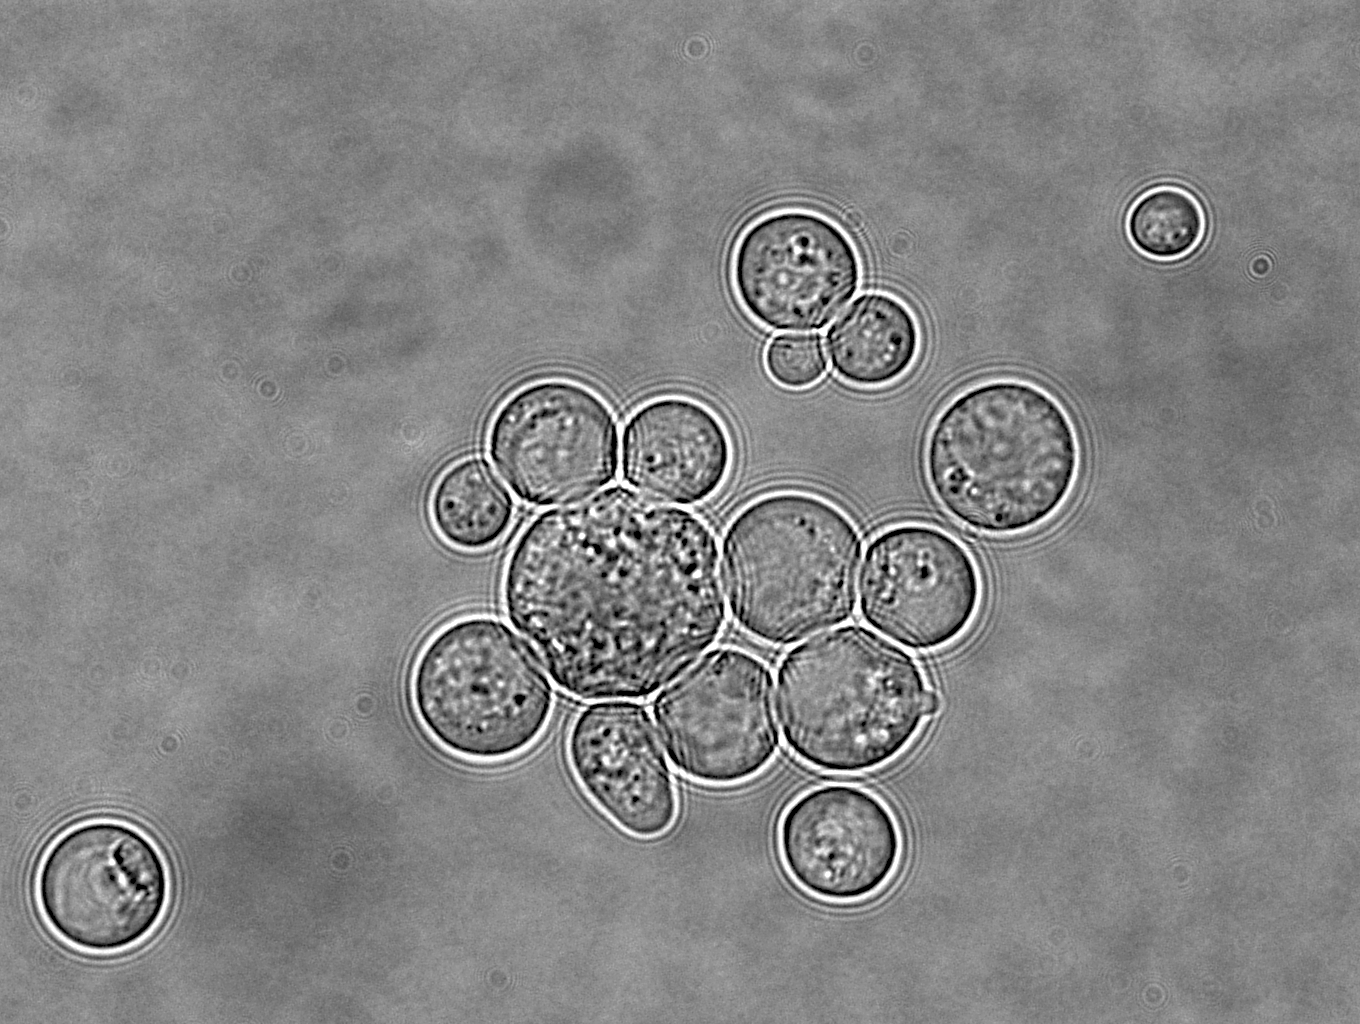
\includegraphics[width = \textwidth]{pics/1246_5hrs_GAL-4-0.png}
		\caption{DIC}\label{fig:}

	\end{subfigure}
	\begin{subfigure}[t]{0.49\linewidth}
		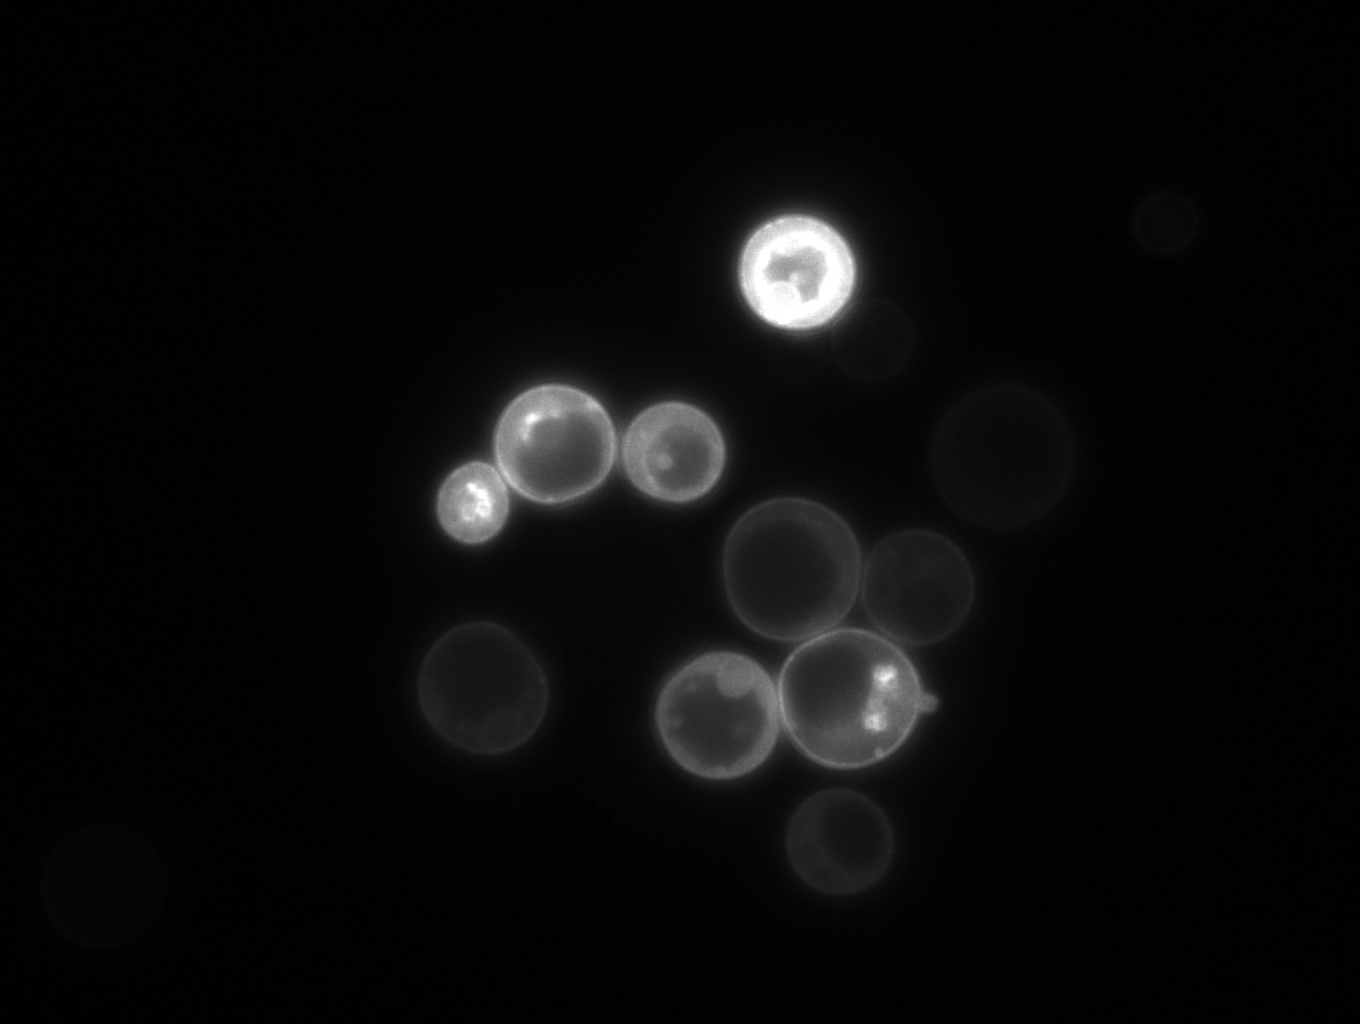
\includegraphics[width = \textwidth]{pics/1246_5hrs_GAL-4-1.png}
		\caption{Флуюресценция}\label{fig:}
	\end{subfigure}

	\caption{Экспрессия α-синуклеина-GFP штаммом W303/αSyn после индукции на галактозе в течении 5 часов.}
	\label{fig:fluo}	
\end{figure*}


\begin{figure*}[h]
	\centering

	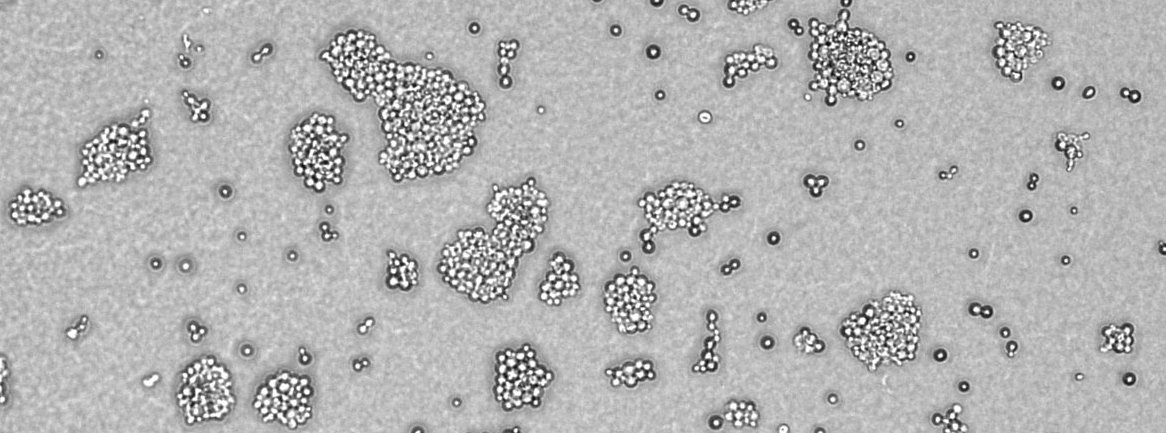
\includegraphics[width = 0.7\textwidth]{pics/16_4_1246_5_nghts_-uraGAL.jpg}
	\caption{Штамм W303/αSyn после культивирования на галактозе в течение 5 суток.}
	\label{fig:division}	
\end{figure*}

%\begin{figure*}[h]
%	\centering
%	\begin{subfigure}[t]{0.49\textwidth}
%		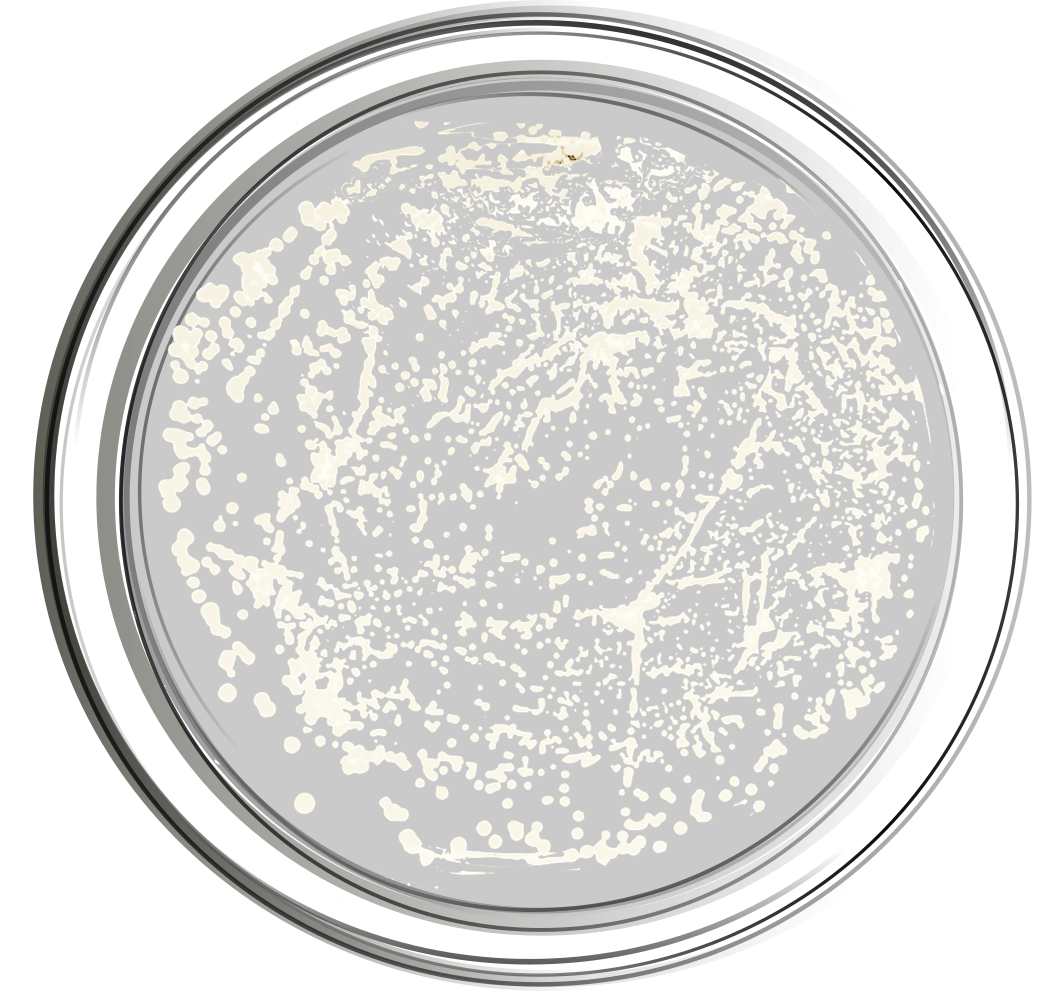
\includegraphics[width = \textwidth]{pics/1158_4n_glu_bw.png}
%		\caption{YNB-uraD}\label{fig:glu}
%
%	\end{subfigure}
%	\begin{subfigure}[t]{0.49\linewidth}
%		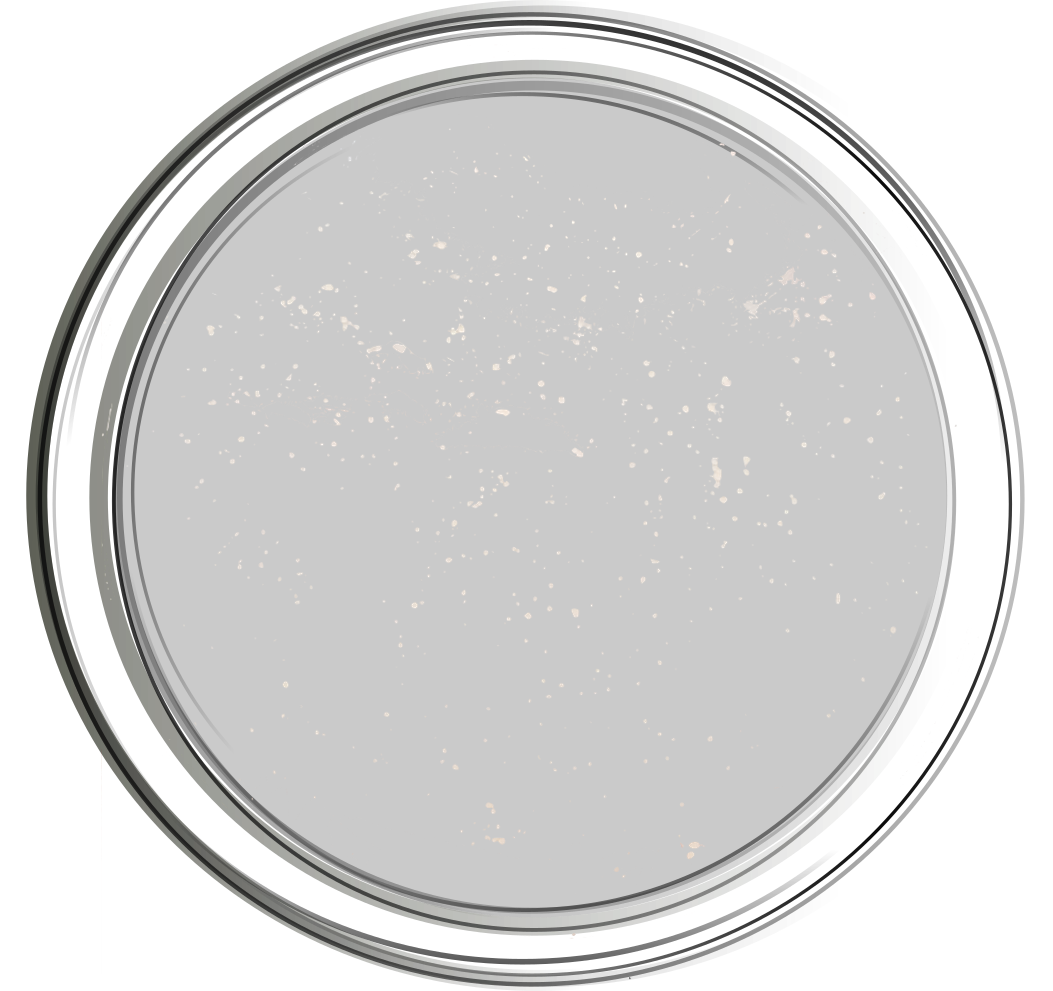
\includegraphics[width = \textwidth]{pics/1158_4n_gal_bw.png}
%		\caption{YNB-uraGAL}\label{fig:gal}
%	\end{subfigure}
%
%	\caption{
%	Рост штамма W303/αSyn: культивирование в течение 4 суток на средах: (a) с глюкозой и \ref{fig:gal} индуцирующей с галактозой. На глюкозе штамм формирует крупные колонии,на галактозе -- мелкие и в меньшем количестве. 
%	\gray{Картинки были созданы из фотографий чашек петри с помощью графических редакторов с сохранением формы и размера колоний для качественной иллюстрации}.
%		}
%	\label{fig:compare}	
%\end{figure*}



Оверэкспрессионная библиотека была трансформирована в штамм  W303/αSyn. Но не было получено ни одного клона. Трансформацию повторили, также с другими клонами W303/αSyn и штаммом, содержащим аналогичную плазмиду pYES-DA-6. При этом аналогичная процедура трансформации успешно проходила с дрожжами дикого типа W303 и штаммом W303:URA3.

Чем могло быть вызвано такое поведение штаммов W303/αSyn? Во-первых, какими-то процедурными неточностямии и ошибками, которые мы не смогли выявить. Во-вторых, мы предположили, что клетки не могут по каким-то причинам удержать обе плазмиды, которые мы хотели поместить в них, так они высококопийные. 

%Тогда мы решили интегрировать плазмиду p426GALaSynGFP и аналогичную по маркёру URA3 плазмиду pYES-DA-6 в геном дрожжей (см. \ref {subsec:integration}). 
%Было проанализировано 20 клонов для плазмиды p426GAlaSynGFP, 10 для плазмиды pYES-DA-6 с помощью ПЦР. Дополнительно, некоторые клоны были трансформировали оверэкспрессионной библиотекой. В результате клонов с встроившейся плазмидой и/или транформирующихся библиотекой найдено не было.
%Для преодоления данного препятствия было предложено несколько путей решения. Один из них заключался в использовании диплоидного штамма, клетки которого больше, содержат больше ДНК, в которых количественно больше машинерии для содержания ДНК-плазмид. Второй способ заключался с переносе интересующей конструкции в центромерную плазмиду pRS314. Эта плазмида в клетке реплицируется наряду с хромосомами и обычно очень низкокопийна.

Для решения этой проблемы было опробовано несколько подходов: (1) интеграция плазмид в геном, (2) проверка совмести мости плазмида с библиотекой в диплоидном штамме, (3) проверка совместимости плазмидного скелета pRS314 с оверэкспрессионной библиотекой.


%Диплоидный штамм был трансформирован плазмидой p426GAlaSynGFP, отобраны клоны, которые далее были транформированы оверэкспрессионной библиотекой, эффективность 60\,клонов/мкл.

%Плазмида pRS314, пока без интересующей конструкции, также были трансформирована в дрожии дикого типа W303, полученные клоны далее трансформированы оверэкспрессионной библиотекой, эффективность 30\,клонов/мкл.

Был заново проведен поиск клона W303/αSyn с более высоким уровнем токсичности α-синуклеина, выбран новый клон W303/αSyn, который, как оказалось, трансформировался оверэкспрессионной библиотекой.

Делеционная библиотека эффективно трансформировалась в штаммы.

Таким образом, мы получили штаммы W303/αSyn, cdc53-1/αSyn, которые экспрессируют α-синуклеин на галактозе, α-синуклеин для них токсичен и образует включения в клетках, которые трансформируются геномными библиотеками.




\subsection{Подбор стратегии скрининга для поиска генетических элементов, вовлеченных в токсичность α-синуклеина в дрожжах}

Мы планировали проводить скрининги на выживание на галактозе. После трансформации геномных библиотек в штаммы планировалось подобрать условия  процедуры так, чтобы после индукции экспрессии α-синуклеина, отбиралось около 0.1-0.5\% трансформантов. Более жесткие условия могли бы нивелировать разницу между разными моделями. С другой стороны, необходимо было понизить уровень ложно-положительных результатов -- отбора клонов, которые не получили никакого генетического преимущества и выросли случайно. Было предложено два варианта проведения скрининга -- с перепечатыванием и с непосредственнным высеванием на индуцирующую среду (см.~\ref{subsec:screening_strats})


Вариант процедуры скрининга с перепечатыванием был протестирован на штамме W303/αSyn с использованием делеционной библиотеки (см.~\ref{subsec:printing}).

Оказалось, что предложенный способ имеет недостатки: (1) размер колоний при перепечатывании очень важен, слишком мелкие колонии сложно все перенести на новую чашку, переросшие же колонии создают неравномерность -- разное количество клеток может быть перенесено, что может очень сильно повлиять на дальнейший рост, что противоречит выбранному критерию отбора; (2) после переноса доля выросших клонов оказалась слишком высокой -- около 10\% -- что говорит о неэффективности процедуры.

Был выбран второй вариант скрининга с непосредственным высеванием на индуцирующую среду (см.~\ref{subsec:immidiately}).

В рамках тестового скрининга мы провели серию транcформаций со штаммами W303/αSyn и cdc53-1/αSyn (при 25°C и 37°C). 
 В таблице~\ref{table:clones_stat} приведены: доля клонов, которые отбирались на галактозе, достигнутое покрытие генома при первичном отборе, предположительная клонов для проверки для полного покрытия генома.


\begin{table}[h]
	\caption{Характеристика первичного отбора, дотигнутого в скринингах.}
	\label{table:clones_stat}
	\begin{tabular}{
		p{0.2\width - \tabcolsep} 
		p{0.2\width - 2\tabcolsep} 
		R{0.2\width - 2\tabcolsep} 
		R{0.2\width - 2\tabcolsep}
		R{0.2\width - \tabcolsep}
		}
	\graytable
	\toprule
	 Штамм & Библиотека & Доля отбираемых клонов & Покрыто генома при первичном отборе & Клонов для проверки всего \\
	\midrule
	W303/αSyn & оверэкс. & 0,4\% & 75\%  & 40 \\
	W303/αSyn & делец. & 0,15\% & 7\% & 45 \\
	cdc53-1/αSyn & оверэкс. & 5\% & 10\% & 500\\
	cdc53-1/αSyn & оверэкс. (тепловой~шок) & 0,7\% & 45\% & 70\\
	\bottomrule
	\end{tabular}
\end{table}


Стоит заметить, что крупные колонии на галактозных чашках после трансформации W303/αSyn появлялись медленно, становились видимыми после 2 суток культивирования, отсаживались после 3-4.
В экспериментах с штаммом cdc53-1/αSyn это время было больше -- около 5-7  дней, так как штамм растет сам по себе очень медленно. После теплового больше колонии появились через 10 суток.
%Полученное время достаточно велико -- за него может произойти множество перестроек в клетке, которые мы не сможем оценить. Поэтому доверять большим колониям после 10 суток культивирования может быть неразумно.

%Выбранный критерий отбора оказался достаточно жестким в экспериментах со штаммом W303/αSyn, но для штамма cdc53-1/αSyn критерий оказался слишком мягким, так как доля отбираемых клонов составляет >0.5\%. 
%Поэтому условия скрининга для штамма cdc53-1/αSyn требуют ужесточения.

Итак, мы остановились на варианте проведения скрининга с непосредственным высеванием на индуцирующую среду. 

\subsection{Проверка клонов, прошедших отбор при скрининге}

Для дальнейшего анализа отобранных трансформантов нам было необходимо убедиться, что эффект повышения выживаемости значителен, воспроизводим и обусловлен делецией или оверэкспрессией какого-либо гена. 

%Воспроизводимость для оверэкспрессионной библиотеки можно было бы проверить выделением плазмиды, ее амплификацией, повторной трансформацией в дрожжи, проверкой.



Клоны, отобранные в результате трансформации штамма W303/αSyn оверэкспрессионной библиотекой были проверены на выживаемость и наличие GFP в клетке (см.~\ref{subsec:second_check}).

% Мы оценивали их скорость росте на галактозе по сравнению со штаммом W303/αSyn/LEU2 (негативный контроль) и W303::URA3/LEU2 (позитивный контроль), а также светимость GFP после индукции экспрессии. Было проверено 30 клонов. Оказалось, что не потерявшие целевую плазмиду клоны сильно уступают в скорости роста штамму W303::URA3/LEU2, и растут в некоторых случаях незначительно лучше W303/αSyn/LEU2. Один клон показал восстановление выживаемости, но он потерял токсичную плазмиду p426GALaSynGFP.


На данный момент нам не удалось обнаружить клонов, которые бы показали значительное и воспроизводимое повышение выживаемости. Было проверено 30 клонов для штамма W303/αSyn и оверэкспрессионной библиотеки, что покрывает около 75\% генома штамма.

Получается, что условия скрининга для штамма W303 оказались слишком жесткими, так при покрытии генома 75\% генетических элементов, повышающих выживаемость при экспрессии синуклеина найдено не было. 


\section{Выводы}


\begin{itemize}[label={--}]
	
\item был подготовлен ДНК-материал для трансформаций дрожжей \emph{Saccharomyces cerevisiae} -- оверэкспрессионная и делеционная дрожжевые геномные библиотеки;
\item созданы штаммы дрожжей \emph{Saccharomyces cerevisiae} W303 и cdc53-1 с индуцибельной экспрессией гибридного белка α-синуклеина-GFP;
\item показано, что α-синуклеин токсичен для штаммов W303 и cdc53-1;
%\item отработаны различные методики трансформации дрожжей;
\item начат скрининг, покрыто 75\% генома для штамма W303/αSyn и оверэкспрессионной библиотеки, клонов найдено не было;
\item показано, что условия скрининга нуждаются, с одной стороны, в смягчении, а с другой стороны -- в повышении эффективности поиска.
\end{itemize}






 




 \newpage
        \footnotesize \bibliographystyle{mybib5.bst}  % стилевой файл для оформления по ГОСТу  utf8gost705u, ieeetr для курсовой, cell  -- черновик
        \bibliography{bib.bib}
\end{document}
